\documentclass[conference]{IEEEtran}
\usepackage{cite}
\usepackage{amsmath,amssymb}
\usepackage{graphicx}
\usepackage{textcomp}
\usepackage{xcolor}
\usepackage{booktabs}
\usepackage{array}
\usepackage{url}
\usepackage{tikz}
\usetikzlibrary{positioning}
\usepackage[english,spanish]{babel}
\addto\captionsspanish{\renewcommand{\tablename}{Tabla}}
\usepackage{listings}
% Fuente monoespaciada estándar (CM): evita que \texttt{} salga vacío si falta Courier (pcrr7t) en la instalación de TeX.
\renewcommand{\ttdefault}{cmtt}
\setlength{\emergencystretch}{2em}
\lstset{basicstyle=\ttfamily\scriptsize,breaklines=true,columns=fullflexible,frame=single,showstringspaces=false,aboveskip=4pt,belowskip=4pt}

\begin{document}

\title{Implementación de aprendizaje automático para la clasificación y caracterización del tráfico de red, Trujillo, 2026}

\author{
\IEEEauthorblockN{Ortega Pinillos Luis Patricio}
\IEEEauthorblockA{Escuela de Ingeniería Informática\\
Universidad Nacional de Trujillo\\
Trujillo, Perú\\
t012700220@unitru.edu.pe}
\and
\IEEEauthorblockN{Vértiz Palomino Akira Mikael}
\IEEEauthorblockA{Escuela de Ingeniería Informática\\
Universidad Nacional de Trujillo\\
Trujillo, Perú\\
avertizp@unitru.edu.pe}
}

\maketitle

\renewcommand{\abstractname}{Resumen}
\begin{abstract}
La creciente proporción de tráfico de red cifrado limita la utilidad de los métodos de clasificación basados en puertos estáticos o en la inspección directa del contenido. Este trabajo propone un sistema de aprendizaje automático supervisado para clasificar y caracterizar tráfico de red a partir de características observables de flujo, con dos dimensiones de análisis: clasificación por tipo de aplicación o servicio y caracterización orientada a seguridad. El sistema se plantea como una aplicación web con API de inferencia, entrenada sobre conjuntos de datos públicos etiquetados. Se reportan dos experimentos independientes: clasificación binaria de seguridad con CICIDS2017, donde Random Forest alcanzó 98,16\,\% de F1 macro en prueba sin información de puertos (con 98 ataques no detectados), y clasificación de siete categorías de aplicación con ISCXVPN2016, donde Gradient Boosting alcanzó 86,24\,\% de F1 macro. La agregación de predicciones sobre los conjuntos de prueba se verificó localmente; el despliegue en la nube y la captura propia permanecen pendientes. Se documentan explícitamente los límites de identificación, de generalización y de interpretación de seguridad del sistema propuesto.
\end{abstract}

\renewcommand{\IEEEkeywordsname}{Palabras clave}
\begin{IEEEkeywords}
aprendizaje automático, clasificación de tráfico de red, tráfico cifrado, aprendizaje supervisado, caracterización de tráfico
\end{IEEEkeywords}

\vspace{0.5em}

\renewcommand{\abstractname}{Abstract}
\begin{abstract}
\foreignlanguage{english}{The growing share of encrypted network traffic limits the usefulness of classification methods based on static ports or direct content inspection. This work proposes a supervised machine learning system to classify and characterize network traffic from observable flow features, along two dimensions of analysis: classification by application or service type, and security-oriented characterization. The system is designed as a web application with an inference API, trained on labeled public datasets. Two independent experiments are reported: binary security classification on CICIDS2017, where Random Forest reached a 98.16\,\% test macro-F1 without port information (with 98 undetected attacks), and seven-class application classification on ISCXVPN2016, where Gradient Boosting reached an 86.24\,\% macro-F1. Prediction aggregation over the test sets was verified locally; cloud deployment and the self-collected capture remain pending. The identification, generalization, and security-interpretation limits of the proposed system are explicitly documented.}
\end{abstract}

\renewcommand{\IEEEkeywordsname}{Keywords}
\begin{IEEEkeywords}
machine learning, network traffic classification, encrypted traffic, supervised learning, traffic characterization
\end{IEEEkeywords}

\section{Introducción}

\subsection{Realidad problemática}

La utilización cotidiana de computadoras depende de numerosas aplicaciones y servicios que mantienen comunicaciones de red en segundo plano, desde navegación y reproducción de contenido hasta sincronización, actualización de software, mensajería y almacenamiento remoto. Para la administración de una red, conocer qué tipos de tráfico atraviesan una conexión ayuda a comprender el uso de recursos, caracterizar servicios y apoyar tareas de seguridad. La literatura sobre clasificación de tráfico considera precisamente la inferencia de aplicaciones y servicios a partir de sus comunicaciones como una actividad relevante para la gestión de redes, la monitorización y la obtención de información de perfilado sobre el comportamiento del tráfico \cite{shen2023,aceto2021}.

Una dificultad práctica aparece cuando la información disponible se encuentra distribuida entre numerosas conexiones pequeñas y heterogéneas. Observar cada flujo de forma independiente puede producir una gran cantidad de registros cuya interpretación resulta difícil para una persona, especialmente cuando el computador mantiene varias aplicaciones abiertas y múltiples servicios operan simultáneamente. En ese escenario, una clasificación individual puede adquirir valor adicional cuando se transforma en información agregada: cantidad de flujos por categoría, volumen aproximado de bytes, frecuencia de determinadas clases o evolución temporal del tráfico. Esta representación no sustituye el análisis detallado de una red, pero permite pasar de una lista de conexiones a una descripción sintética del comportamiento observado.

El perfilado agregado también puede apoyar la administración cotidiana. Permite observar qué actividades concentran tráfico y facilita interpretar cambios de distribución entre navegación, streaming, juegos, almacenamiento o actualizaciones sin revisar cada conexión. Un aumento poco habitual o la aparición de flujos fuera de las clases conocidas puede justificar una revisión posterior, pero no convierte una clasificación estadística en una afirmación determinista sobre la identidad o intención de una comunicación.

El problema se vuelve más complejo cuando las comunicaciones utilizan protocolos cifrados. Los métodos tradicionales de clasificación basados únicamente en puertos conocidos o en la inspección profunda del contenido pierden parte de su utilidad cuando el tráfico se transporta mediante HTTPS, TLS, VPN u otros mecanismos que ocultan el contenido de aplicación. Estudios recientes señalan que esta transformación ha impulsado el uso de características estadísticas, temporales y de secuencia de paquetes para intentar inferir la aplicación o servicio asociado a un flujo sin necesidad de inspeccionar directamente su contenido \cite{shen2023,ahmed2021,roy2022,zaki2022}.

La clasificación de tráfico no se limita a distinguir aplicaciones. Las redes también deben enfrentar comunicaciones cuyo comportamiento puede ser inesperado o estar asociado a actividades potencialmente no deseadas. La literatura muestra que la selección y representación de características, la distribución de las clases y la presencia de tráfico no visto pueden afectar el desempeño de los clasificadores \cite{shen2023,jin2024,liang2024,afuwape2021,pathmaperuma2022}.

En este contexto, una herramienta que produzca una caracterización agregada del tráfico podría aportar una representación comprensible del uso de red de un equipo. En lugar de mostrar cientos o miles de conexiones aisladas, el sistema podría consolidar los resultados en categorías de servicio y mostrar qué proporción de flujos o bytes corresponde a navegación web, streaming, juegos, mensajería o almacenamiento. En paralelo, una segunda dimensión experimental podría utilizar un único conjunto de datos de seguridad para estudiar, de forma separada, categorías definidas por ese dataset. Así, la caracterización de aplicaciones y la clasificación de seguridad se mantienen como tareas diferenciadas y no se mezclan sus espacios de características ni sus etiquetas.

La agregación también puede servir como referencia descriptiva para comparar periodos de uso. Un cambio de distribución, como la aparición de una categoría no habitual o un aumento de conexiones en un grupo concreto, no demuestra por sí mismo un incidente, pero puede justificar una revisión posterior. El sistema se orientará así al apoyo de la observación, manteniendo explícitos sus límites de interpretación.

No obstante, existen limitaciones que deben incorporarse desde el planteamiento. Una dirección IP no identifica de manera permanente una aplicación o un servicio: distintos servicios pueden compartir infraestructura, las direcciones pueden cambiar y una misma aplicación puede utilizar múltiples proveedores. Del mismo modo, la presencia de un dominio observado mediante DNS no garantiza que toda la comunicación posterior pueda atribuirse de manera exclusiva a ese dominio. Por ello, la propuesta no pretende clasificar direcciones IP como si fueran identidades permanentes, sino clasificar flujos utilizando un conjunto de características observables. La información de IP y, cuando esté disponible, la información DNS de la captura propia se reservarán para aportar contexto y facilitar la interpretación de resultados exploratorios, no como variables de entrada obligatorias del clasificador.

La literatura reciente también advierte sobre la existencia de tráfico desconocido y sobre la dificultad de transferir un modelo entrenado con clases conocidas a aplicaciones o patrones que no estaban presentes durante el entrenamiento \cite{liang2024,pathmaperuma2022}. Esto es especialmente relevante para una aplicación que pretenda funcionar sobre el tráfico cotidiano de un computador, donde pueden existir aplicaciones no incluidas en el conjunto de entrenamiento. Por esta razón, la propuesta contempla separar claramente la evaluación sobre datos etiquetados de la observación exploratoria de tráfico real, evitando presentar esta última como una prueba de exactitud si no existe una verdad de referencia suficiente.

La situación problemática puede resumirse, por tanto, en la dificultad de obtener una caracterización automática y estructurada del tráfico de red a partir de observables de flujo, especialmente en escenarios donde el contenido está cifrado y donde pueden coexistir servicios conocidos, aplicaciones desconocidas y comportamientos potencialmente no deseados. La aplicación de aprendizaje automático ofrece un mecanismo para aprender patrones a partir de datos etiquetados y producir clasificaciones que luego pueden agregarse para formar un perfil de uso de red \cite{shen2023,aceto2021,roy2022}. El reto de la investigación no será demostrar una identificación absoluta de cada conexión, sino determinar hasta qué punto un conjunto acotado de características permite obtener clasificaciones útiles y reproducibles dentro de un alcance experimental claramente delimitado.

\subsection{Problema de investigación}

\textbf{¿Cómo clasificar y caracterizar el tráfico de red mediante aprendizaje automático a partir de características observables de los flujos de comunicación?}

Problemas específicos de apoyo a la investigación:
\begin{itemize}
\item ¿Qué características observables de un flujo resultan útiles para distinguir categorías de aplicación o servicio?
\item ¿Qué desempeño presentan distintos algoritmos de aprendizaje automático al clasificar las categorías seleccionadas?
\item ¿Cómo se comporta un clasificador entrenado con datos públicos cuando se aplica a tráfico generado durante el uso cotidiano de un computador?
\item ¿Qué información puede obtenerse al agregar las clasificaciones individuales para construir un perfil de tráfico?
\end{itemize}

\subsection{Justificación}

\textbf{Justificación académica.} La investigación permitirá profundizar en el estudio del aprendizaje supervisado aplicado a la clasificación de tráfico de red, integrando conceptos de representación de datos, ingeniería de características, entrenamiento, validación y evaluación de clasificadores. Asimismo, permitirá estudiar las dificultades particulares de la clasificación de tráfico cifrado, como el uso de características estadísticas y temporales, las diferencias entre niveles de granularidad y la aparición de tráfico desconocido \cite{shen2023,jin2024,liang2024,afuwape2021,pathmaperuma2022}.

\textbf{Justificación tecnológica.} La propuesta traduce un problema de análisis de redes en una aplicación informática desplegable. El sistema puede separar la fase experimental, donde se preparan datos y se entrenan y comparan modelos, de la fase de servicio, donde un modelo seleccionado expone predicciones mediante una API y una interfaz web. Esto hace viable cumplir el requisito de despliegue en la nube sin convertir la infraestructura de producción en el objeto central de la investigación.

\textbf{Justificación práctica.} Una caracterización agregada del tráfico puede facilitar la interpretación del uso de red de un equipo o conjunto de flujos. En lugar de observar exclusivamente conexiones individuales, el usuario puede consultar categorías de aplicaciones o servicios, volumen de tráfico y observaciones de seguridad. El proyecto se enfocará en apoyo a la observación y caracterización, no en reemplazar mecanismos profesionales de seguridad.

\textbf{Justificación social.} Una caracterización agregada puede beneficiar a usuarios y administradores de redes pequeñas, como hogares, laboratorios universitarios o pequeñas empresas, que carecen de herramientas profesionales de monitoreo, al mostrarles de forma comprensible qué servicios concentran su tráfico. Al trabajar solo con metadatos de flujo y evitar almacenar el contenido de las comunicaciones, la propuesta favorece además una observación de red respetuosa de la privacidad.

\textbf{Justificación metodológica.} El uso combinado de un conjunto de datos público etiquetado y una colección independiente de tráfico cotidiano permite diferenciar dos escenarios: evaluación controlada del clasificador y observación exploratoria en condiciones de uso real. Esta separación ayuda a evitar que una evaluación sin etiquetas sea presentada como una medición de exactitud. Además, el empleo de una estrategia de partición agrupada busca reducir el riesgo de fuga de información entre entrenamiento y prueba, aspecto especialmente importante cuando registros de una misma sesión o captura pueden compartir patrones fuertemente relacionados.

\textbf{Relación con los Objetivos de Desarrollo Sostenible (ODS).} El trabajo se vincula principalmente con el ODS 9, que busca construir infraestructuras resilientes, promover una industrialización inclusiva y fomentar la innovación \cite{ods9}. La clasificación y caracterización de tráfico es una capacidad de gestión de la infraestructura de comunicaciones y el proyecto la aborda con datos públicos y herramientas abiertas, de modo que pueda replicarse en entornos con recursos limitados. De forma secundaria, se relaciona con el ODS 16, cuyo propósito incluye construir instituciones eficaces, responsables y transparentes \cite{ods16}, en la medida en que una mejor observación del tráfico puede apoyar la seguridad de los servicios digitales de organizaciones pequeñas. Esta segunda vinculación es indirecta: el prototipo no es una política pública y no se ha medido ningún efecto social, por lo que no se atribuyen impactos cuantificados.

\subsection{Objetivos}

\textbf{Objetivo general.} Implementar un sistema de aprendizaje automático para clasificar y caracterizar el tráfico de red a partir de características observables de los flujos de comunicación.

\textbf{Objetivos específicos.}
\begin{enumerate}
\item Identificar y preparar un conjunto de datos etiquetado de tráfico de red, seleccionando las características observables de flujo que permitan representar las categorías de clasificación estudiadas.
\item Entrenar y comparar algoritmos de aprendizaje automático para la clasificación de las categorías de tráfico seleccionadas.
\item Evaluar el desempeño de los modelos mediante métricas de clasificación y análisis de errores.
\item Implementar y desplegar una API/aplicación web que utilice el modelo seleccionado para clasificar flujos de red en la nube.
\item Diseñar un mecanismo de agregación que consolide las clasificaciones individuales en una caracterización global del tráfico analizado.
\end{enumerate}

\subsection{Marco teórico}

\subsubsection{Antecedentes}

\textbf{Shen et al. \cite{shen2023}.} Presentan una revisión amplia de la clasificación y el análisis de tráfico cifrado mediante aprendizaje automático. Los autores organizan el área según diferentes objetivos de análisis, entre ellos la identificación de activos de red, la caracterización de la red, la detección de fugas de privacidad y la detección de anomalías, y sintetizan un flujo metodológico que comprende la recopilación del tráfico, su representación, el método de análisis y la evaluación del desempeño. La revisión muestra que la clasificación no es un problema único, sino una familia de tareas con distintos niveles de granularidad y necesidades de información. Para la presente propuesta, este antecedente aporta una base para ubicar la clasificación de aplicaciones y servicios dentro del análisis de tráfico cifrado y, a la vez, justificar la necesidad de separar la caracterización de tráfico de otros objetivos de seguridad. La brecha que se retoma consiste en traducir ese marco general a un prototipo experimental de alcance acotado, con características de flujo observables, modelos relativamente simples y una etapa posterior de agregación de resultados.

\textbf{Ahmed y Agunsoye \cite{ahmed2021}.} Proponen NetScrapper, un clasificador de tráfico basado en flujos para aplicaciones en línea. El sistema considera atributos como conteo y tamaño de paquetes, tiempos entre llegadas y relaciones entre tráfico enviado y recibido, y utiliza tres modelos de aprendizaje automático --K-Nearest Neighbors, Random Forest y una red neuronal artificial-- para distinguir un conjunto amplio de aplicaciones. Además del componente de clasificación, los autores implementan una interfaz web que permite cargar datos de tráfico y una modalidad de captura desde la interfaz de red, conectando los modelos con un middleware desarrollado sobre Flask. La evaluación considera métricas de desempeño de clasificación y tiempo de predicción, por lo que constituye un antecedente directo de la integración entre modelo y aplicación. Sin embargo, su objetivo y cobertura son más amplios que los necesarios para el presente proyecto. La brecha que se adopta aquí es reducir el espacio experimental a categorías manejables y concentrar la investigación en la relación entre representación de flujo, desempeño del modelo y caracterización agregada, manteniendo la aplicación web como resultado de despliegue y no como sustituto del análisis experimental.

\textbf{Aceto et al. \cite{aceto2021}.} Presentan DISTILLER, una arquitectura de aprendizaje profundo multimodal y multitarea para la clasificación de tráfico cifrado. El enfoque combina distintas modalidades de representación del tráfico y utiliza un esquema multitarea para resolver simultáneamente tareas de clasificación relacionadas. La motivación central del trabajo es que los flujos cifrados aún contienen patrones estadísticos y secuenciales que pueden utilizarse para inferir aplicaciones o servicios, aunque el contenido no esté disponible para inspección directa. Su evaluación se plantea mediante comparación con arquitecturas de referencia de aprendizaje profundo y permite observar el efecto de integrar representaciones diferentes. Este trabajo respalda el supuesto general de que la información observable de un flujo puede ser suficiente para la clasificación, pero también evidencia que las arquitecturas multimodales pueden alcanzar una complejidad considerable. La propuesta actual responde a esa tensión mediante un alcance deliberadamente más pequeño, priorizando modelos tabulares y una representación de características de flujo que pueda ser reproducida y desplegada con recursos moderados.

\textbf{Roy, Shapira y Shavitt \cite{roy2022}.} Estudian la clasificación rápida de tráfico cifrado utilizando dos características elementales de los flujos: tamaño de los paquetes y tiempos entre llegadas. Su propuesta emplea un modelo basado en Neural ODE para representar la evolución temporal de los estados del flujo y plantea una evaluación con conjuntos balanceados para facilitar comparaciones más confiables entre clases. Un aspecto relevante es la intención de obtener una clasificación temprana, utilizando una cantidad relativamente pequeña de observaciones del flujo, en lugar de esperar a disponer de una captura extensa. El trabajo demuestra que la clasificación puede apoyarse en información estrictamente estadística y temporal, sin acceso al contenido del paquete. Para la presente investigación, este antecedente refuerza la elección de metadatos de flujo como base de representación y aporta una referencia para discutir eficiencia. La brecha específica es que nuestro proyecto no busca optimizar la clasificación temprana mediante una arquitectura especializada, sino evaluar un pipeline de características y modelos clásicos que pueda integrarse de manera sencilla en una aplicación de perfilado.

\textbf{Zaki et al. \cite{zaki2022}.} Proponen GRAIN, un enfoque de clasificación granular y multietiqueta que distingue niveles de aplicación y servicio mediante una cadena de clasificadores. En particular, la propuesta enlaza dos clasificadores Random Forest: el primero identifica el nombre de la aplicación y su salida se incorpora como información para el segundo, que determina categorías de servicio a un nivel más detallado. La representación inicial utiliza características estadísticas construidas a partir de la longitud de los datos del tráfico, evitando depender del contenido de los paquetes y manteniendo su utilidad cuando existe cifrado. La evaluación se orienta a demostrar la capacidad de distinguir categorías con distinta granularidad y a conservar las interdependencias entre etiquetas. Este antecedente es especialmente útil porque muestra que la noción de ``clasificar una aplicación'' puede separarse conceptualmente de la de ``caracterizar el servicio''. La presente propuesta adopta esa distinción, pero restringe el nivel de detalle a categorías que puedan sostenerse con el dataset disponible y evita convertir la granularidad jerárquica en una exigencia innecesaria para el prototipo.

\textbf{Li et al. \cite{li2023}.} Proponen FusionTC para la clasificación de tráfico de aplicaciones cifrado y organizan el procesamiento en unidades de flujo. Su arquitectura emplea dos niveles de subclasificadores y una estrategia de fusión a nivel de decisión que combina representaciones multimodales de la secuencia de tráfico. El propósito es aprovechar información complementaria cuando un único tipo de característica no representa adecuadamente patrones complejos del tráfico. La evaluación se realiza sobre un conjunto de datos de tráfico de aplicaciones construido por los propios autores y compara el rendimiento con enfoques de referencia. Este antecedente aporta evidencia de que la información temporal y estadística de un flujo puede ser combinada de distintas maneras y de que la representación tiene un efecto importante sobre el resultado final. A la vez, su arquitectura demuestra un nivel de complejidad mayor al requerido para un proyecto de un semestre. La propuesta actual responde a esa brecha con una representación tabular más simple y con comparación de modelos clásicos, de modo que la contribución experimental sea comprensible y reproducible sin implementar un sistema multimodal profundo.

\textbf{Jin et al. \cite{jin2024}.} Estudian la clasificación de tráfico cifrado mediante un enfoque de aprendizaje federado y distinguen explícitamente dos tareas: la identificación de aplicaciones y la caracterización del tráfico por categorías de servicio. El estudio utiliza el conjunto ISCXVPN2016 y considera escenarios en los que distintas partes del tráfico se distribuyen entre participantes, empleando una red convolucional unidimensional como modelo base del aprendizaje federado. La evaluación compara el esquema federado con configuraciones de aprendizaje centralizado y permite observar cómo la clasificación puede mantenerse cuando la información de tráfico no se concentra en un único participante. Para el presente proyecto, su principal relevancia no está en reproducir el aprendizaje federado, sino en la coincidencia entre sus dos tareas de clasificación y la organización conceptual planteada aquí. La brecha consiste en estudiar el mismo problema desde una arquitectura centralizada mucho más sencilla, orientada a la comparación de modelos y al perfilado agregado, sin introducir los costos técnicos propios de la coordinación federada.

\textbf{Liang et al. \cite{liang2024}.} Proponen STI, un sistema de identificación de tráfico con mecanismos orientados a aplicaciones desconocidas y basado en una versión mejorada de Random Forest. El problema de partida es que una gran cantidad de tráfico real no coincide necesariamente con las clases disponibles durante el entrenamiento, por lo que un sistema de identificación debe considerar la presencia de datos que no corresponden a las categorías conocidas. La investigación incorpora esta situación como parte explícita del problema y analiza la capacidad del sistema para reconocer tráfico conocido y tratar tráfico desconocido. Este antecedente es relevante porque conecta directamente el desempeño de un modelo de clasificación con el entorno abierto de una red real, donde las aplicaciones evolucionan y aparecen comportamientos que no estaban presentes al construir el dataset. La presente investigación no intentará implementar un sistema completo de descubrimiento de clases desconocidas; en cambio, utilizará el tráfico cotidiano como observación exploratoria y tratará el problema de generalización como una limitación que debe analizarse a partir de los resultados obtenidos.

\textbf{Afuwape et al. \cite{afuwape2021}.} Evalúan técnicas de aprendizaje automático para la clasificación de tráfico protegido y estudian tanto modelos individuales como métodos de conjunto. El trabajo incluye experimentación sobre un problema de clasificación de tráfico P2P y analiza el comportamiento de modelos en escenarios asociados con redes VPN, utilizando medidas de desempeño para comparar las alternativas. Esta orientación es útil para la presente propuesta porque muestra que la comparación entre algoritmos debe realizarse bajo un protocolo común y que la selección del modelo final puede sustentarse con evidencia experimental en lugar de asumirse previamente. También aporta un antecedente para discutir la relación entre precisión de clasificación y características del dominio protegido. La brecha que aborda este proyecto consiste en trasladar esa lógica comparativa a un conjunto de categorías de aplicación o servicio más delimitado y complementar la evaluación con análisis de errores y posterior agregación de las predicciones para el perfil de tráfico.

\textbf{Pathmaperuma et al. \cite{pathmaperuma2022}.} Estudian la clasificación de tráfico cifrado y la detección de datos desconocidos mediante una red neuronal profunda. Su propuesta utiliza una representación basada en ventanas temporales para dividir el tráfico de una actividad en segmentos y emplea la distribución de salida del modelo para distinguir entre actividades aprendidas y observaciones que no pertenecen a las clases utilizadas durante el entrenamiento. La evaluación analiza tanto la identificación de actividades conocidas como el tratamiento de actividades no vistas, lo que permite estudiar el problema desde una perspectiva distinta a la clasificación cerrada tradicional. Este antecedente refuerza la necesidad de diferenciar entre clasificación de clases conocidas y comportamiento ante datos fuera del dominio. En el proyecto actual, esa distinción se utilizará para interpretar con cautela los resultados sobre tráfico cotidiano: las observaciones propias podrán mostrar cómo se comporta el modelo frente a condiciones distintas del benchmark, pero no se transformarán automáticamente en una métrica de exactitud.

\textbf{Pacheco et al. \cite{pacheco2019}.} Presentan una revisión sistemática sobre el despliegue de soluciones de aprendizaje automático en la clasificación de tráfico, organizada según los pasos necesarios para construir un clasificador. Los autores parten de que el cifrado y la encapsulación reducen el rendimiento de las estrategias clásicas y señalan tendencias y direcciones futuras del área. Este antecedente respalda la estructura por etapas adoptada en el proyecto (datos, características, modelo, evaluación y puesta en servicio) y recuerda que el paso de un resultado experimental a un sistema operativo exige validación adicional. La brecha que se retoma es documentar, con evidencia verificable, qué etapas del proceso se completaron en un proyecto de alcance acotado y cuáles permanecen pendientes.

\textbf{Rezaei y Liu \cite{rezaei2019}.} Ofrecen una visión general de la clasificación de tráfico cifrado con aprendizaje profundo e introducen un marco general de siete pasos que va desde la formulación del problema hasta la actualización periódica del modelo. Definen el flujo mediante la tupla de cinco elementos (direcciones IP, puertos y protocolo) y advierten que, para la mayoría de los problemas de tráfico, no existe un conjunto de datos aceptado de forma común. Para la presente investigación, el trabajo aporta una justificación de la separación entre preparación de datos, selección de características, entrenamiento y validación, y refuerza la necesidad de declarar la procedencia de cada dataset. A diferencia de ese enfoque, este proyecto compara modelos clásicos sobre características tabulares ya calculadas.

\textbf{Ring et al. \cite{ring2019}.} Realizan una revisión de conjuntos de datos para detección de intrusiones en red y proponen quince propiedades, agrupadas en cinco categorías, para evaluar la idoneidad de cada conjunto en un escenario concreto, junto con recomendaciones para su uso y creación. Este antecedente fundamenta que CICIDS2017 se trate como un benchmark con propiedades y límites explícitos, y no como una muestra representativa de cualquier red. La brecha que se aborda es traducir esas recomendaciones a decisiones concretas de muestreo, partición y exclusión de variables.

\textbf{Engelen et al. \cite{engelen2021}.} Revisan CICIDS2017 y su proceso de recolección y detectan problemas en la generación de tráfico, la construcción de flujos, la extracción de características y el etiquetado; reportan que más del 20\,\% de las trazas originales fue reconstruido o reetiquetado. Para este proyecto, el trabajo es una advertencia metodológica: los archivos GeneratedLabelledFlows se usan tal como se distribuyen, sin aplicar las correcciones propuestas, por lo que los resultados deben leerse como desempeño sobre ese benchmark y no como una medida de la detección de ataques reales.

\textbf{Rosay et al. \cite{rosay2022} y Lanvin et al. \cite{lanvin2022}.} Rosay et al. analizan los CSV de CIC-IDS2017 y encuentran problemas como la duplicación de características y errores en su cálculo; Lanvin et al. identifican fallos en el etiquetado y en la captura (desorden y duplicación de paquetes, y ataques ejecutados pero no etiquetados). Estos antecedentes justifican dos decisiones del proyecto: eliminar la columna duplicada \texttt{Fwd Header Length.1} de cada archivo y tratar los resultados como desempeño sobre el benchmark tal como se distribuye, sin afirmar detección real de ataques.

\textbf{Kurniabudi et al. \cite{kurniabudi2020}.} Analizan la selección de características de CICIDS-2017 mediante ganancia de información y evalúan Random Forest, Bayes Net, Naive Bayes, Random Tree y J48; concluyen que el número de características relevantes influye en la exactitud y el tiempo de ejecución. Es el antecedente más cercano a la comparación entre 69 y 68 características de este trabajo, que difiere en que no usa ganancia de información sino la exclusión explícita de puertos y protocolo.

\textbf{Apruzzese et al. \cite{apruzzese2023}.} Analizan el papel del aprendizaje automático en ciberseguridad y señalan que su despliegue práctico se encuentra en una etapa temprana, con una brecha entre los resultados de investigación y la práctica. El trabajo es relevante porque sitúa las métricas de un benchmark como evidencia necesaria pero insuficiente. El presente proyecto adopta esa cautela al discutir falsos negativos y al evitar afirmar preparación para producción.

\textbf{Grinsztajn et al. \cite{grinsztajn2022}.} Comparan modelos de aprendizaje profundo y modelos basados en árboles en un conjunto de 45 datasets tabulares y encuentran que los modelos de árboles siguen siendo competitivos o superiores en datos de tamaño medio (del orden de diez mil muestras). Este resultado orienta la comparación del proyecto, cuyos datasets de entrenamiento tienen decenas de miles de registros, y ofrece un marco para interpretar por qué el MLP no superó a Random Forest ni a Gradient Boosting.

\subsubsection{Conceptos y fundamentos teóricos}

\textbf{Aprendizaje automático.} Disciplina que permite construir modelos que aprenden patrones a partir de datos para realizar tareas como clasificación, regresión o detección de anomalías. En esta propuesta se utilizará aprendizaje supervisado porque las observaciones de entrenamiento dispondrán de etiquetas de clase \cite{geron2022,bishop2024}.

\textbf{Aprendizaje supervisado y contraste con aprendizaje no supervisado.} En el aprendizaje supervisado cada observación se acompaña de una etiqueta que representa la salida esperada, de modo que el modelo ajusta sus parámetros a partir de ejemplos donde la relación entre entradas y clases está definida. En contraste, los métodos no supervisados buscan estructuras o agrupamientos sin disponer de una etiqueta objetivo previamente proporcionada. Para este proyecto, la clasificación principal requiere aprendizaje supervisado debido a que ISCXVPN2016 y el dataset de seguridad seleccionado ofrecen clases que permiten construir un problema de entrenamiento y evaluación. La distinción resulta importante porque una eventual observación de tráfico cotidiano sin etiquetas no constituye por sí misma un conjunto de prueba supervisado \cite{geron2022,bishop2024}.

\textbf{Clasificación supervisada.} Problema en el que cada instancia de entrada se asocia con una clase conocida durante el entrenamiento. Para el proyecto, la entrada corresponderá a un flujo o representación agregada del tráfico y la salida a una categoría de aplicación, servicio o comportamiento previamente definida \cite{geron2022,bishop2024}.

\textbf{Ingeniería y selección de características.} Proceso de transformar datos observados en variables que representen de manera útil los patrones que un modelo debe aprender, así como de elegir un subconjunto de variables relevantes para la tarea. En tráfico de red, esta etapa puede involucrar medidas de duración, paquetes, bytes, tamaños y relaciones temporales. Una representación adecuada puede reducir complejidad, facilitar el entrenamiento y evitar introducir variables que no estarán disponibles de forma consistente durante la inferencia \cite{geron2022,bishop2024}. La selección será especialmente importante en esta investigación porque el uso de información presente solamente en una fuente de datos y ausente en otra produciría una metodología difícil de reproducir.

\textbf{Flujo de red.} Unidad lógica de observación formada por una secuencia de paquetes que comparten características de comunicación, normalmente delimitadas por direcciones, puertos, protocolo y actividad temporal. Trabajar con flujos reduce el problema a registros estructurados y facilita el uso de algoritmos de aprendizaje sobre datos tabulares \cite{ahmed2021,roy2022}. Los puertos y el protocolo identifican, en las capas de transporte y aplicación, los extremos de la comunicación y el servicio asociado \cite{kurose2021}, lo que explica que su uso como variables pueda dar información dependiente del escenario de captura y no del comportamiento del tráfico.

\textbf{Características de flujo.} Variables observables que describen la comunicación sin necesidad de utilizar directamente el contenido de aplicación, como duración, cantidad de paquetes, bytes enviados y recibidos, tamaños de paquetes, tasa de transmisión y tiempos entre paquetes. Las investigaciones recientes muestran que estas características pueden servir como representación para clasificación \cite{shen2023,ahmed2021,roy2022,li2023}.

\textbf{Clasificación por aplicación o servicio.} Proceso de inferir la categoría de aplicación o servicio asociada a un flujo. La literatura distingue niveles diferentes de granularidad, desde familias generales hasta nombres de aplicaciones o servicios específicos \cite{aceto2021,zaki2022}. Para el proyecto se propone comenzar con categorías manejables y evitar una granularidad que no pueda sostenerse con datos suficientes.

\textbf{Clasificación de seguridad.} Proceso de asignar a un flujo una clase relacionada con comportamiento benigno, anómalo o una categoría de ataque definida en el conjunto de datos. Esta dimensión será tratada de manera independiente a la clasificación de aplicación y no se utilizará para afirmar que una conexión constituye malware por sí sola \cite{sharafaldin2018,moustafa2015}.

\textbf{Tráfico cifrado.} Tráfico en el que el contenido de la comunicación se encuentra protegido mediante protocolos criptográficos. La imposibilidad de inspeccionar directamente el contenido motiva el uso de metadatos y características estadísticas para clasificación \cite{shen2023,roy2022,li2023}.

\textbf{Datos desconocidos.} Muestras que no pertenecen a las clases utilizadas durante el entrenamiento. La presencia de aplicaciones o servicios no conocidos es un reto reconocido en la identificación de tráfico \cite{liang2024,pathmaperuma2022}.

\textbf{Matriz de confusión y métricas de evaluación.} En un problema de $K$ clases, la matriz de confusión registra cuántas instancias de cada clase real fueron asignadas a cada clase predicha. Para una clase $c$, con verdaderos positivos $TP_c$, falsos positivos $FP_c$ y falsos negativos $FN_c$, se definen
\begin{align}
P_c &= \frac{TP_c}{TP_c+FP_c}, \qquad R_c = \frac{TP_c}{TP_c+FN_c},\\
F1_c &= \frac{2\,P_c\,R_c}{P_c+R_c}, \qquad \text{Exactitud} = \frac{\sum_c TP_c}{N}.
\end{align}
La precisión indica qué fracción de las predicciones de una clase es correcta; la exhaustividad (\emph{recall}), qué fracción de los casos reales de la clase fue encontrada, y el F1 es su media armónica. El promedio macro, $\frac{1}{K}\sum_c F1_c$, otorga el mismo peso a cada clase; el promedio ponderado pesa cada clase por su soporte $n_c$. Cuando las clases son desbalanceadas, la exactitud puede ofrecer una estimación demasiado optimista, porque está dominada por las clases frecuentes \cite{chicco2020}; por ello, el F1 macro y las métricas por clase permiten ver el desempeño en las clases minoritarias. En seguridad, además, el costo de los dos errores es distinto: un falso negativo es un ataque no detectado y un falso positivo es una alerta innecesaria, por lo que se reporta la tasa de falsos negativos $FN/(FN+TP)$ de forma explícita \cite{ring2019,apruzzese2023}.

\textbf{Regresión logística.} Modelo lineal que estima la probabilidad de pertenencia a una clase mediante la función logística (o su extensión multiclase, softmax). Su bajo costo computacional y su interpretabilidad lo convierten en una línea base habitual \cite{hastie2009,geron2022}.

\textbf{Random Forest.} Conjunto de árboles de decisión entrenados sobre muestras aleatorias de los datos y subconjuntos aleatorios de características, cuya predicción final se obtiene por votación. La aleatorización reduce la varianza del modelo y suele funcionar bien con datos tabulares \cite{hastie2009,geron2022}.

\textbf{Boosting.} Familia de métodos que entrena aprendices débiles de forma secuencial, de modo que cada uno corrige los errores del anterior. Suele lograr alto desempeño en datos tabulares, aunque es más sensible a la configuración de hiperparámetros \cite{hastie2009,geron2022}.

\textbf{Perceptrón multicapa.} Red neuronal en la que cada capa oculta aplica una transformación lineal seguida de una función de activación no lineal (aquí, ReLU), y cuyos pesos se ajustan por descenso de gradiente con retropropagación; el optimizador Adam adapta la tasa de aprendizaje de cada parámetro \cite{bishop2024}. Su capacidad de representación es alta, pero depende de la escala de las variables, de la regularización y de la cantidad de datos, y en datos tabulares de tamaño medio los modelos de árboles suelen igualarlo o superarlo \cite{grinsztajn2022}.

\textbf{Desbalance de clases y fuga de información.} El desbalance ocurre cuando unas clases tienen muchos más ejemplos que otras; sus efectos se mitigan con ponderación de clases, remuestreo o métricas apropiadas \cite{chicco2020,hastie2009}. La fuga de información aparece cuando registros muy relacionados (por ejemplo, flujos de una misma sesión o intervalo temporal) caen en particiones distintas, lo que infla el desempeño estimado; por eso la literatura de aprendizaje automático en seguridad recomienda particiones que separen grupos y evaluaciones realistas \cite{arp2022}.

\textbf{Clasificación de seguridad frente a clasificación de aplicaciones.} Aunque ambas usan flujos y aprendizaje supervisado, difieren en su objetivo y en la naturaleza de sus clases. La clasificación de seguridad distingue tráfico benigno de actividad de ataque definida por el dataset y es sensible al costo de los falsos negativos; la clasificación de aplicaciones asigna cada flujo a una categoría de servicio (navegación, correo, VoIP, etc.) y su dificultad proviene del parecido estadístico entre categorías \cite{shen2023,pacheco2019}. Por ello se tratan como experimentos separados, con sus propias etiquetas, características y métricas.

\textbf{Biblioteca de implementación.} Los modelos y el flujo de preprocesamiento se implementaron con scikit-learn \cite{pedregosa2011}, cuyas clases \texttt{LogisticRegression}, \texttt{RandomForestClassifier}, \texttt{HistGradientBoostingClassifier} y \texttt{MLPClassifier} corresponden a los algoritmos comparados.

\textbf{Perfil de tráfico.} Representación agregada de las clasificaciones obtenidas durante un periodo. Puede incluir número de flujos, bytes, distribución por categorías y proporción de tráfico observado. Su función en el proyecto será descriptiva, no una prueba de identidad absoluta de aplicaciones \cite{shen2023}.

\subsubsection{Fuentes de datos consideradas}

La Tabla~\ref{tab:fuentes} resume las fuentes de datos consideradas, su función dentro de la investigación y las precauciones metodológicas asociadas a cada una.

\begin{table*}[!t]
\centering
\caption{Fuentes de datos consideradas y su función en la investigación}
\label{tab:fuentes}
\begin{tabular}{p{2.6cm}p{3.4cm}p{4.6cm}p{5.4cm}}
\toprule
\textbf{Fuente} & \textbf{Función en la investigación} & \textbf{Ventaja} & \textbf{Precaución} \\
\midrule
Dataset público etiquetado de clasificación de tráfico & Entrenamiento, validación y evaluación controlada. & Permite disponer de etiquetas y comparar modelos. & Debe analizarse su distribución de clases y su correspondencia con el alcance del proyecto. \\
Dataset público de tráfico de seguridad & Evaluación de la dimensión de seguridad en clases seleccionadas. & Incluye clases benignas y de actividad maliciosa/ataques. & No debe combinarse con el dataset de aplicaciones en un mismo espacio de características; se evalúa como tarea independiente. \\
Captura propia de uso cotidiano & Evaluación exploratoria y construcción de un perfil de tráfico. & Representa tráfico generado fuera del benchmark. & La etiqueta real de cada flujo puede no ser conocida; no se usará para afirmar exactitud sin un protocolo adicional de verdad de referencia. \\
\bottomrule
\end{tabular}
\end{table*}

\textbf{Datasets seleccionados.} Para la clasificación de aplicaciones y servicios se utilizará ISCXVPN2016 \cite{drapergil2016}. Los archivos disponibles para esta tarea se encuentran en formato ARFF, por lo que antes del entrenamiento se inspeccionarán sus declaraciones de atributos, tipos de variables y etiquetas de clase. El formato contiene una declaración de relación (\texttt{@RELATION}), declaraciones de atributos (\texttt{@ATTRIBUTE}) y los registros de datos (\texttt{@DATA}). Se utilizará un lector compatible con los tipos que efectivamente aparezcan: \texttt{scipy.io.arff.loadarff} permite leer atributos numéricos y nominales, mientras que los archivos con atributos de texto, fecha o datos dispersos requieren un parser que soporte esos tipos. Los valores nominales se decodificarán y se conservarán como etiquetas categóricas; después se convertirá el contenido a una representación tabular compatible con el pipeline de aprendizaje automático. La conversión no supondrá que todos los archivos contienen las mismas columnas: primero se verificará la correspondencia de atributos y categorías entre archivos. También se documentará la procedencia exacta de los ARFF recibidos, dado que la ficha institucional de ISCXVPN2016 describe las capturas PCAP y los flujos CSV generados con ISCXFlowMeter (\url{https://www.unb.ca/cic/datasets/vpn.html}); por tanto, los ARFF deben identificarse como una representación procesada o conversión de esa fuente. Para la clasificación de seguridad se seleccionó CICIDS2017, específicamente los archivos de flujos etiquetados de GeneratedLabelledFlows, que incluyen marcas temporales necesarias para formar grupos de diez minutos. Ambos conjuntos se procesarán y evaluarán como tareas independientes; no se combinarán sus registros, características ni etiquetas.

\textbf{Naturaleza de los conjuntos de referencia.} CICIDS2017 fue creado para caracterizar tráfico de intrusión y contiene flujos benignos y de varias familias de ataque con características estadísticas extraídas por flujo \cite{sharafaldin2018}; su uso extendido convive con observaciones sobre errores de generación y de etiquetado \cite{engelen2021}. ISCXVPN2016 describe tráfico cifrado y VPN mediante características basadas en tiempo, calculadas sobre ventanas de duración fija \cite{drapergil2016}. Ambos son conjuntos de referencia, útiles para comparar métodos bajo condiciones controladas, pero no equivalen a tráfico de producción \cite{ring2019}.

\textbf{Captura propia y anotación contextual.} La colección propia de varias horas de tráfico cotidiano tendrá una finalidad exploratoria. El flujo observado se describirá mediante sus metadatos y, cuando la captura lo permita, podrá relacionarse con eventos de DNS para facilitar la interpretación cualitativa de algunas conexiones. Esta información contextual no formará parte del conjunto de características de entrada del modelo, ya que no se encuentra disponible de forma equivalente en los datasets públicos utilizados para la evaluación. De este modo, la observación de tráfico real servirá para construir el perfil agregado y examinar ejemplos fuera del benchmark sin introducir una variable que solo existiría en una parte de la investigación.

\subsubsection{Modelo conceptual de la propuesta}

El sistema se plantea como una cadena de procesamiento en la que el dato primario es el flujo de red y el resultado es una clasificación acompañada de información agregada:

La Figura~\ref{fig:pipeline} resume la cadena de procesamiento.

\begin{figure}[!t]
\centering
\resizebox{\columnwidth}{!}{%
\begin{tikzpicture}[node distance=0.35cm, box/.style={draw, rounded corners=2pt, minimum height=0.9cm, text width=1.5cm, align=center, font=\scriptsize, fill=blue!8}]
\node[box] (a) {Tráfico de red};
\node[box, right=of a] (b) {Extracción de características};
\node[box, right=of b] (c) {Modelo ML};
\node[box, right=of c] (d) {Clasificación};
\node[box, right=of d] (e) {Agregación y perfil};
\foreach \x/\y in {a/b,b/c,c/d,d/e} \draw[-latex] (\x) -- (\y);
\end{tikzpicture}}
\caption{Cadena de procesamiento propuesta.}
\label{fig:pipeline}
\end{figure}

La primera etapa transforma las comunicaciones en registros y prepara las variables disponibles para el modelo. El clasificador asigna una categoría a cada flujo como predicción estadística, y el mecanismo de agregación resume los resultados mediante conteos, volumen de bytes o distribución por categoría.

La arquitectura separa dos tareas experimentales independientes. La clasificación por aplicación o servicio se entrenó y evaluó sobre ISCXVPN2016, mientras que la clasificación de seguridad se desarrolló sobre CICIDS2017, con su propio espacio de características, preparación y etiquetas. Así se evita tratar como equivalentes variables y resultados obtenidos en dominios diferentes.

En la captura propia podrán conservarse IP y, cuando sea posible, eventos DNS para interpretación y anotación cualitativa. DNS no será una característica del clasificador y una IP no se asumirá como identidad de una aplicación. El flujo central seguirá basado en características observables y será reproducible con el dataset público de evaluación.

La propuesta se completa con una capa de servicio que expone el modelo mediante una API y una interfaz web. Esta capa recibe datos de flujo estructurados, aplica el mismo preprocesamiento del entrenamiento y retorna la clasificación, que puede agregarse para mostrar el perfil resultante. La nube constituye así el entorno de despliegue, mientras que la comparación de modelos y el análisis de desempeño permanecen como núcleo de la investigación.

\section{Método}

\subsection{Tipo de investigación}
La investigación será de tipo aplicada, debido a que busca utilizar conocimientos y métodos de aprendizaje automático para implementar una solución informática concreta orientada a la clasificación y caracterización de tráfico de red.

\subsection{Enfoque de investigación}
El curso admite como técnicas de inteligencia artificial el aprendizaje automático, las redes bayesianas y los sistemas de inferencia difusa. Este proyecto emplea aprendizaje automático supervisado: clasificadores entrenados con ejemplos etiquetados (Regresión Logística, Random Forest, Gradient Boosting y perceptrón multicapa) \cite{hastie2009,bishop2024}; no se emplean redes bayesianas ni sistemas de inferencia difusa.

El enfoque será cuantitativo, porque se trabajará con datos estructurados de tráfico y se medirán resultados mediante indicadores numéricos como precisión, recall, F1-score, exactitud, tiempo de inferencia y distribución de errores por clase.

\subsection{Diseño de investigación}
Se propone un diseño experimental, dado que se manipulará de manera controlada la configuración del proceso de entrenamiento y comparación de modelos y se observará su efecto sobre métricas de clasificación. La experimentación se realizará sobre datos etiquetados y se mantendrán separados el conjunto de entrenamiento y el conjunto de prueba. En una fase complementaria se observará tráfico cotidiano sin confundir dicha observación exploratoria con una medición supervisada de exactitud.

\textbf{Estrategia de partición entrenamiento/validación/prueba.} Para reducir el riesgo de fuga de información se aplicó el siguiente procedimiento \cite{arp2022}: (1) eliminación de registros exactamente duplicados antes de la partición (no se buscaron casi duplicados); (2) en el experimento de seguridad con CICIDS2017, partición aleatoria por grupos temporales de diez minutos (\texttt{TimeGroup}), de modo que los flujos de un mismo intervalo no aparezcan en más de una partición; (3) en el experimento de aplicaciones con ISCXVPN2016, partición aleatoria estratificada por clase, porque el ARFF seleccionado no incluye identificador de sesión ni marca temporal; (4) registro de los tamaños efectivos de cada partición. En ambos casos el programa separa primero la prueba y después la validación del bloque restante. Al repartir grupos y no registros, las proporciones reales difieren de las nominales (Sección~\ref{sec:programa}). La partición por intervalos de diez minutos no constituye una evaluación cronológica entre días ni garantiza que campañas de ataque similares queden aisladas; la partición estratificada de ISCXVPN2016 no impide que flujos de una misma captura estén en entrenamiento y prueba.


\subsection{Variables de estudio}

La Tabla~\ref{tab:variables} presenta las variables del estudio, su rol y los indicadores propuestos para cada una.

\begin{table*}[!t]
\centering
\caption{Variables de estudio}
\label{tab:variables}
\begin{tabular}{p{3.6cm}p{2.8cm}p{9.6cm}}
\toprule
\textbf{Variable} & \textbf{Rol} & \textbf{Dimensiones / indicadores propuestos} \\
\midrule
Características observables del tráfico de red & Variable de entrada / independiente & Duración del flujo; paquetes enviados/recibidos; bytes enviados/recibidos; tasas; tamaños estadísticos de paquetes; tiempos entre llegadas; protocolo; puertos; estado de conexión; información DNS asociada cuando esté disponible en la captura propia (usada únicamente como anotación contextual, no como entrada del clasificador). \\
Clasificación del tráfico de red & Variable de salida / dependiente & Categoría de aplicación/servicio; categoría de seguridad; clase desconocida/no contemplada cuando el diseño permita evaluarla. \\
Desempeño del modelo de clasificación & Variable de resultado & Accuracy; precision; recall; F1-score; matriz de confusión; tiempo de inferencia; comportamiento por clase. \\
\bottomrule
\end{tabular}
\end{table*}

\subsection{Población y muestra}
\textbf{Población.} Conjunto de flujos de tráfico de red generados por aplicaciones, servicios y comportamientos de comunicación que puedan observarse mediante registros o capturas de red durante el periodo de estudio.

\textbf{Muestra.} Conjunto de flujos etiquetados seleccionados de los datasets públicos para las clases definidas en el estudio y, de manera complementaria, registros obtenidos de una captura propia de varias horas de uso cotidiano del computador. La muestra exacta se determinará después de inspeccionar la distribución de clases y la disponibilidad real de datos.

\subsection{Técnicas e instrumentos}

La Tabla~\ref{tab:tecnicas} relaciona las técnicas de recolección y análisis con los instrumentos empleados y su uso previsto.

\begin{table*}[!t]
\centering
\caption{Técnicas e instrumentos}
\label{tab:tecnicas}
\begin{tabular}{p{3.2cm}p{4.8cm}p{7.2cm}}
\toprule
\textbf{Técnica} & \textbf{Instrumento / fuente} & \textbf{Uso} \\
\midrule
Observación estructurada & Registros de flujo generados por una herramienta de captura/análisis de red (p. ej. Zeek). & Recolectar atributos de flujo y observar la distribución del tráfico cotidiano. Cuando esté disponible, el registro DNS (\texttt{dns.log}) se emplea únicamente para anotar e interpretar de forma cualitativa los resultados de la captura propia, no como característica de entrada del modelo. \\
Análisis documental & Datasets públicos, artículos científicos y documentación técnica. & Seleccionar clases, variables, procedimientos y antecedentes para el diseño experimental. \\
Experimentación computacional & Scripts de preprocesamiento, entrenamiento y evaluación. & Entrenar modelos y medir su desempeño bajo condiciones controladas, incluyendo la partición agrupada entrenamiento/prueba. \\
\bottomrule
\end{tabular}
\end{table*}

\subsection{Procedimiento propuesto}
\begin{enumerate}
\item Definir las categorías de aplicación/servicio y las categorías de seguridad que sean sostenibles con los datasets elegidos.
\item Descargar, revisar y documentar los datasets públicos; comparar explícitamente su espacio de características y esquema de etiquetas; identificar valores faltantes, duplicados y desbalance de clases.
\item Seleccionar las características que serán utilizadas por los modelos y establecer un pipeline reproducible de limpieza y transformación.
\item Construir conjuntos de entrenamiento, validación y prueba mediante partición agrupada, evitando fuga de información entre particiones.
\item Entrenar y comparar cuatro algoritmos de aprendizaje supervisado: Regresión Logística, Random Forest, HistGradientBoosting y un perceptrón multicapa (MLP), sin asumir de antemano qué modelo obtendrá el mejor desempeño.
\item Evaluar los modelos mediante precision, recall, F1-score, accuracy como métrica complementaria y matriz de confusión.
\item Seleccionar el modelo para el prototipo a partir de criterios documentados de desempeño, costo computacional e interpretabilidad.
\item Recolectar una captura propia de varias horas de tráfico cotidiano para observar cómo se comporta el sistema fuera del benchmark. Las observaciones sin etiqueta se presentarán como análisis exploratorio, apoyado de forma opcional por anotación DNS cuando la captura lo permita.
\item Construir una API de inferencia y una interfaz web que permitan cargar registros o datos de flujo y visualizar clasificaciones y agregaciones.
\item Desplegar la aplicación en la nube y documentar el procedimiento de ejecución y las limitaciones del sistema.
\end{enumerate}
Los pasos 1 a 7 se ejecutaron para ambos experimentos y se documentan en la sección de Resultados. Los pasos 8 a 10 (captura propia, API e interfaz, y despliegue en la nube) permanecen pendientes o parcialmente implementados, como se detalla en las Secciones~\ref{sec:res_app} y~\ref{sec:res_agreg}.

\subsection{Criterios de evaluación}

La Tabla~\ref{tab:criterios} resume los indicadores de desempeño y su interpretación en el contexto del estudio.

\begin{table*}[!t]
\centering
\caption{Criterios de evaluación}
\label{tab:criterios}
\begin{tabular}{p{3.4cm}p{3.2cm}p{8.6cm}}
\toprule
\textbf{Aspecto} & \textbf{Indicador} & \textbf{Interpretación} \\
\midrule
Desempeño global & Accuracy & Proporción de predicciones correctas; se reportará como indicador complementario. \\
Desempeño por clase & Precision & Proporción de predicciones positivas que pertenecen realmente a la clase. \\
Capacidad de detección & Recall & Proporción de instancias de una clase que el modelo logra identificar. \\
Equilibrio entre precision y recall & F1-score & Media armónica de precision y recall por clase. \\
Errores de clasificación & Matriz de confusión & Permite identificar qué clases tienden a confundirse. \\
Viabilidad de la aplicación & Tiempo de inferencia y consumo básico de recursos & Ayuda a determinar si el modelo seleccionado es razonable para el prototipo desplegado. \\
\bottomrule
\end{tabular}
\end{table*}

\section{Atención a las observaciones de la primera entrega}

Las observaciones formuladas por el docente sobre la primera entrega no formaban parte del material de trabajo con el que se preparó esta versión; por ello no se declaran como atendidas y la Tabla~\ref{tab:feedback} deja su registro para completarlo con el texto original. Las modificaciones realizadas por iniciativa de los autores se listan por separado y no sustituyen esa respuesta.

\begin{table}[!tb]
\centering
\footnotesize
\caption{Registro de observaciones y respuesta}
\label{tab:feedback}
\begin{tabular}{p{2.3cm}p{3.7cm}p{1.2cm}}
\toprule
\textbf{Observación} & \textbf{Respuesta / justificación} & \textbf{Estado} \\
\midrule
{[Pendiente: transcribir observaciones del docente]} & {[Pendiente]} & Por completar \\
Objetivos y resultados no alineados (revisión propia) & Cinco secciones de Resultados, una por objetivo específico (Tabla~\ref{tab:trazabilidad}). & Atendido \\
Referencias insuficientes para la segunda entrega (revisión propia) & Bibliografía ampliada a 31 fuentes: 25 artículos, 4 libros y 2 de ODS. & Atendido \\
\bottomrule
\end{tabular}
\end{table}

\section{Resultados}
\label{sec:resultados}

Los resultados se organizan en cinco subsecciones, una por objetivo específico (Tabla~\ref{tab:trazabilidad}). Se presentan dos experimentos independientes: clasificación binaria de seguridad con CICIDS2017 (\textit{Benign} frente a \textit{Attack}) y clasificación de siete categorías de aplicación con ISCXVPN2016. Cada uno usa sus propios registros, características, etiquetas y particiones, y sus métricas no se combinan. Las cifras de las Subsecciones~\ref{sec:res_config} y~\ref{sec:res_eval} se contrastaron con los archivos de salida de cada ejecución (\texttt{metricas\_prueba.json}, \texttt{comparacion\_validacion.csv}, \texttt{reporte\_por\_clase.csv} y \texttt{matriz\_confusion.csv}). Los objetivos 4 y 5 cuentan con avances verificables en inferencia local y agregación de los conjuntos de prueba; sin embargo, la ejecución visual de la interfaz, el despliegue público y la caracterización de tráfico operativo siguen pendientes.

\begin{table*}[!t]
\centering
\caption{Trazabilidad entre objetivos específicos, resultados y evidencia}
\label{tab:trazabilidad}
\small
\begin{tabular}{p{4.6cm}p{2.0cm}p{6.6cm}p{2.6cm}}
\toprule
\textbf{Objetivo específico} & \textbf{Sección} & \textbf{Evidencia} & \textbf{Estado} \\
\midrule
1. Identificar y preparar el conjunto de datos & \ref{sec:res_datos} & Perfil y distribución de clases de ambos datasets; scripts de preparación. & Cumplido \\
2. Entrenar y comparar algoritmos & \ref{sec:res_config} & Configuración de cuatro modelos, programa de entrenamiento y validación, comparación en validación. & Cumplido \\
3. Evaluar el desempeño & \ref{sec:res_eval} & Métricas de prueba, matrices de confusión, métricas por clase y tiempos de predicción. & Cumplido \\
4. Implementar y desplegar API/aplicación web & \ref{sec:res_app} & Dos modelos reales cargados; paridad completa; API local con HTTP 200; 13 pruebas aprobadas. UI y despliegue público pendientes. & Parcial; despliegue pendiente \\
5. Diseñar la agregación & \ref{sec:res_agreg} & Conteos y porcentajes de etiquetas predichas sobre los conjuntos de prueba, resumidos en la Tabla~\ref{tab:agregacion_prueba} y la Figura~\ref{fig:agregacion}. Sin captura propia ni métricas de bytes. & Parcial \\
\bottomrule
\end{tabular}
\end{table*}

\subsection{Construcción y descripción de los conjuntos de datos}
\label{sec:res_datos}

\textbf{Experimento A: CICIDS2017.} Se procesaron ocho archivos CSV de GeneratedLabelledFlows, que incluyen marca temporal y por eso permiten construir grupos temporales; no se usó la versión MachineLearningCSV. El programa \texttt{prepare\_cicids\_generatedflows.py} leyó 3\,119\,345 filas, de las cuales 2\,830\,743 tenían etiqueta no vacía (2\,273\,097 BENIGN y 557\,646 de catorce etiquetas de ataque) y 288\,602 tenían etiqueta vacía y fueron descartadas (Tabla~\ref{tab:cicids_etiquetas}). La etiqueta BENIGN se mapeó a \textit{Benign} y cualquier otra etiqueta no vacía a \textit{Attack}. Algunos archivos contienen bytes de codificación Windows-1252, por lo que el programa intenta UTF-8, Windows-1252 y Latin-1 en ese orden.

\begin{table}[!tb]
\centering
\footnotesize
\caption{Etiquetas originales de CICIDS2017 (filas leídas)}
\label{tab:cicids_etiquetas}
\begin{tabular}{lr}
\toprule
\textbf{Etiqueta original} & \textbf{Registros} \\
\midrule
BENIGN & 2\,273\,097 \\
DoS Hulk & 231\,073 \\
PortScan & 158\,930 \\
DDoS & 128\,027 \\
DoS GoldenEye & 10\,293 \\
FTP-Patator & 7\,938 \\
SSH-Patator & 5\,897 \\
DoS slowloris & 5\,796 \\
DoS Slowhttptest & 5\,499 \\
Bot & 1\,966 \\
Web Attack -- Brute Force & 1\,507 \\
Web Attack -- XSS & 652 \\
Infiltration & 36 \\
Web Attack -- Sql Injection & 21 \\
Heartbleed & 11 \\
\midrule
Etiqueta vacía (descartada) & 288\,602 \\
\textbf{Total de filas leídas} & \textbf{3\,119\,345} \\
\bottomrule
\end{tabular}
\end{table}

En la preparación se eliminó, en cada uno de los ocho archivos, la columna \texttt{Fwd Header Length.1}, tras comprobar que era idéntica a \texttt{Fwd Header Length} (ocho columnas en total). Se construyó la variable \texttt{TimeGroup} redondeando la marca temporal a intervalos de diez minutos; las filas sin marca temporal interpretable se agruparían por archivo; \texttt{perfil\_dataset.json} reporta 0 filas sin marca temporal interpretable en los archivos fuente. El muestreo tomó hasta 10\,000 registros por clase y por archivo, unió las muestras, eliminó duplicados exactos de esa muestra intermedia y limitó cada clase final a 20\,000 registros, con semilla 42 (\texttt{--per-class-per-file 10000 --max-per-class 20000 --group-minutes 10}). El perfil reporta 0 filas duplicadas eliminadas de esa muestra intermedia, y \texttt{train\_validate.py}, que también elimina duplicados exactos, conservó los 40\,000 registros. Antes del límite final, el conjunto candidato tenía 80\,000 flujos benignos (10\,000 por archivo) y 44\,182 de ataque (10\,000 en cada uno de los archivos de DDoS, PortScan, martes y miércoles; 1\,966 los del viernes por la mañana; 2\,180 los de ataques web; 36 los de infiltración; y ninguno el lunes), de los que se tomaron 20\,000 de cada clase al azar. Por ello la composición por familia de ataque depende de estos límites, y las familias con pocos registros (Heartbleed, Infiltration) tienen una representación esperada muy baja en la muestra final. Los valores infinitos se convierten en faltantes para la imputación posterior.

La Tabla~\ref{tab:dias} muestra la composición de la muestra final por día de captura (derivada de \texttt{TimeGroup}). Los rótulos de fecha de \texttt{TimeGroup} aparecen con día y mes invertidos respecto de la fecha real (por ejemplo, 2017-03-07 corresponde al lunes 3 de julio de 2017, único día sin ataques), lo que no altera la agrupación en intervalos. La muestra final tiene 249 grupos temporales, de entre 3 y 4\,216 registros (mediana de 63).

\begin{table}[!tb]
\centering
\footnotesize
\caption{CICIDS2017: muestra final por día de captura (julio de 2017)}
\label{tab:dias}
\begin{tabular}{lrr}
\toprule
\textbf{Día} & \textbf{Attack} & \textbf{Benign} \\
\midrule
Lunes 3 & 0 & 2\,531 \\
Martes 4 & 4\,568 & 2\,500 \\
Miércoles 5 & 4\,480 & 2\,513 \\
Jueves 6 & 1\,009 & 4\,955 \\
Viernes 7 & 9\,943 & 7\,501 \\
\midrule
\textbf{Total} & \textbf{20\,000} & \textbf{20\,000} \\
\bottomrule
\end{tabular}
\end{table}

La proporción de ataques varía mucho entre días (0\,\% el lunes y 57\,\% el viernes), de modo que la clase está correlacionada con el momento de captura; esto es un sesgo del dataset que la exclusión de puertos no elimina.

El conjunto preparado tiene 40\,000 registros (20\,000 \textit{Benign} y 20\,000 \textit{Attack}), 85 columnas y 79 columnas numéricas candidatas. En el entrenamiento se excluyen los identificadores y marcas de tiempo (por patrón de nombre), la variable \texttt{TimeGroup}, y las columnas que el programa descarta por tener menos de 50\,\% de valores numéricos o ninguna variación. En la primera configuración se excluyeron además \texttt{Source Port} y \texttt{Protocol}, y se conservó \texttt{Destination Port}, lo que dejó 69 características. En la segunda se excluyeron \texttt{Source Port}, \texttt{Destination Port} y \texttt{Protocol}, con 68 características. De 79 a 69 características hay diez columnas menos: dos corresponden a las exclusiones explícitas y, por diferencia, se infiere que ocho fueron descartadas por el filtro automático (inferencia: \texttt{configuracion.json} registra las columnas excluidas por patrón y por \texttt{--drop-cols}, pero no las eliminadas por el filtro automático).

\textbf{Experimento B: ISCXVPN2016.} Se inspeccionaron los ocho ARFF de Scenario B (ventanas de 15, 30, 60 y 120 s, cada una en variante normal y \texttt{AllinOne}) y se seleccionó \texttt{TimeBasedFeatures-Dataset-60s-AllinOne.arff}, que contiene 15\,516 registros y 24 atributos: 23 características numéricas y una etiqueta nominal, \texttt{class1}, con siete categorías. La variante \texttt{AllinOne} agrupa las variantes VPN y no VPN de cada categoría, por lo que la tarea es clasificación de aplicaciones o servicios y no detección de VPN. La conversión (\texttt{iscx\_arff\_tool.py convert}) omitió un registro con etiqueta vacía y produjo 15\,515 registros, con las etiquetas normalizadas a Browsing, Chat, FileTransfer, Mail, P2P, Streaming y VoIP. Al leer el CSV para entrenar, \texttt{train\_validate.py} eliminó 817 filas exactamente duplicadas mediante \texttt{drop\_duplicates()}, de modo que el conjunto efectivo fue de 14\,698 registros. La Tabla~\ref{tab:iscx_clases} muestra la distribución convertida y el soporte en prueba, y la Tabla~\ref{tab:estructura} resume la estructura final de ambos conjuntos.

\begin{table}[!tb]
\centering
\footnotesize
\caption{Clases de ISCXVPN2016 (60 s, AllinOne)}
\label{tab:iscx_clases}
\begin{tabular}{lrrr}
\toprule
\textbf{Clase} & \textbf{Convertidos} & \textbf{\%} & \textbf{Soporte prueba} \\
\midrule
Browsing & 5\,000 & 32,2 & 993 \\
VoIP & 3\,449 & 22,2 & 681 \\
FileTransfer & 2\,270 & 14,6 & 410 \\
P2P & 1\,823 & 11,7 & 320 \\
Chat & 1\,292 & 8,3 & 246 \\
Mail & 1\,232 & 7,9 & 206 \\
Streaming & 449 & 2,9 & 84 \\
\midrule
\textbf{Total} & \textbf{15\,515} & 100 & \textbf{2\,940} \\
\bottomrule
\end{tabular}
\end{table}

\begin{table}[!tb]
\centering
\footnotesize
\caption{Estructura final de los conjuntos usados}
\label{tab:estructura}
\begin{tabular}{p{2.2cm}p{2.5cm}p{2.5cm}}
\toprule
\textbf{Propiedad} & \textbf{CICIDS2017} & \textbf{ISCXVPN2016} \\
\midrule
Tarea & Binaria (Benign/Attack) & 7 clases \\
Registros usados & 40\,000 & 14\,698 \\
Características & 69 y 68 (dos configuraciones) & 23 \\
Distribución & 20\,000 / 20\,000 (balanceada) & Desbalanceada (Tabla~\ref{tab:iscx_clases}) \\
Partición & Por grupos \texttt{TimeGroup} & Estratificada \\
\bottomrule
\end{tabular}
\end{table}

Las limitaciones de ambos conjuntos se discutieron en la Sección~\ref{sec:limitaciones}. En particular, las métricas de CICIDS2017 se refieren a una muestra balanceada y no a la prevalencia natural de ataques, y el desbalance de ISCXVPN2016 motiva el uso de F1 macro y de métricas por clase.

\subsection{Configuración de los modelos y programa de entrenamiento y validación}
\label{sec:res_config}

\textbf{Configuración.} Se compararon cuatro algoritmos supervisados con scikit-learn \cite{pedregosa2011}, todos dentro de un \texttt{Pipeline} con imputación por la mediana (\texttt{SimpleImputer}, \texttt{keep\_empty\_features=True}) y estandarización (\texttt{StandardScaler}). La Tabla~\ref{tab:config_modelos} lista los parámetros fijados en el código; el resto toma los valores por defecto de la versión instalada de scikit-learn, correspondiente a scikit-learn 1.8.0, versión registrada en los modelos serializados. Los parámetros de arquitectura de red solo aplican al MLP: Regresión Logística, Random Forest y Gradient Boosting no tienen capas ni neuronas. La salida del MLP es logística para dos clases y softmax para siete, según el comportamiento documentado de la biblioteca. En \texttt{HistGradientBoostingClassifier}, \texttt{learning\_rate} y \texttt{max\_leaf\_nodes} coinciden con los valores por defecto. La detención temprana por defecto ('auto') se activa con más de 10\,000 muestras: en ISCXVPN2016 no actuó durante la selección (9\,553 registros de entrenamiento), pero sí en el modelo final reajustado con 11\,758 registros, que se detuvo en 73 iteraciones (dato leído del modelo serializado).

\begin{table*}[!t]
\centering
\caption{Configuración de los modelos (parámetros fijados en \texttt{train\_validate.py}; semilla 42)}
\label{tab:config_modelos}
\small
\begin{tabular}{p{2.2cm}p{5.0cm}p{8.6cm}}
\toprule
\textbf{Algoritmo} & \textbf{Clase de scikit-learn} & \textbf{Parámetros fijados} \\
\midrule
Regresión Logística & \texttt{LogisticRegression} & \texttt{max\_iter=1000}; \texttt{\detokenize{class_weight="balanced"}}; \texttt{random\_state=42}. Regularización L2 y \texttt{C} por defecto. \\
Random Forest & \texttt{RandomForestClassifier} & \texttt{n\_estimators=300}; \texttt{\detokenize{class_weight="balanced_subsample"}}; \texttt{min\_samples\_leaf=1}; \texttt{n\_jobs=-1}; \texttt{random\_state=42}. \\
Gradient Boosting & \texttt{HistGradientBoostingClassifier} & \texttt{max\_iter=150}; \texttt{learning\_rate=0.1}; \texttt{max\_leaf\_nodes=31}; \texttt{random\_state=42}. Sin ponderación de clases. \\
MLP\_128\_64 & \texttt{MLPClassifier} & Capas ocultas $(128, 64)$; \texttt{\detokenize{activation="relu"}}; \texttt{\detokenize{solver="adam"}}; \texttt{learning\_rate\_init=0.001}; \texttt{alpha=0.0001} (L2); \texttt{batch\_size=256}; \texttt{max\_iter=200}; \texttt{early\_stopping=True}; \texttt{validation\_fraction=0.15}; \texttt{n\_iter\_no\_change=12}; \texttt{random\_state=42}. \\
\bottomrule
\end{tabular}
\end{table*}

\subsubsection{Programa de entrenamiento y validación}
\label{sec:programa}
La entrada es un CSV con una columna objetivo (\texttt{Label}) y, opcionalmente, una columna de grupo (\texttt{TimeGroup}). El programa elimina filas con etiqueta vacía y duplicados exactos, exige al menos tres registros por clase y excluye columnas identificadoras por patrón de nombre (\textit{Flow ID}, direcciones IP, marcas temporales), la columna de grupo y las indicadas con \texttt{--drop-cols}. Convierte el resto a numérico, reemplaza infinitos por faltantes y conserva las columnas con al menos 50\,\% de valores numéricos y más de un valor distinto. Los tres pasos centrales son:

\begin{enumerate}
\item \textit{Partición.} Con grupo, \texttt{GroupShuffleSplit} (hasta 250 intentos) reserva 20\,\% de los grupos para prueba y 18,75\,\% de los grupos restantes para validación, exigiendo que las clases estén presentes en cada partición; sin grupo, se usa \texttt{train\_test\_split} estratificado con las mismas fracciones. Nominalmente resulta 65/15/20 por registros. En ISCXVPN2016 se obtuvo 9\,553/2\,205/2\,940 (65,0/15,0/20,0\,\%). En CICIDS2017, como se reparten grupos de tamaño desigual, se obtuvo 28\,277/5\,766/5\,957 (70,7/14,4/14,9\,\%).
\item \textit{Selección.} Los cuatro modelos se ajustan con la partición de entrenamiento y se evalúan en validación; se elige el de mayor F1 macro (con la exactitud como desempate).
\item \textit{Evaluación final.} El modelo elegido se reajusta con entrenamiento más validación y se evalúa una única vez en prueba. Por tanto, las métricas de validación corresponden a modelos ajustados solo con entrenamiento y las de prueba al modelo reajustado.
\end{enumerate}

{\sloppy El programa genera \texttt{comparacion\_validacion.csv}, \texttt{metricas\_prueba.json}, \texttt{reporte\_por\_clase.csv}, \texttt{matriz\_confusion.csv} y \texttt{.png}, \texttt{predicciones\_prueba.csv}, \texttt{modelo\_entrenado.joblib}, \texttt{caracteristicas.json}, \texttt{etiquetas.json} y \texttt{configuracion.json}. El siguiente fragmento reproduce las partes relevantes del código:\par}

\begin{lstlisting}
Pipeline([("imputacion", SimpleImputer(
    strategy="median", keep_empty_features=True)),
  ("escalado", StandardScaler()),
  ("modelo", estimator)])
RandomForestClassifier(n_estimators=300,
  class_weight="balanced_subsample", n_jobs=-1,
  random_state=seed, min_samples_leaf=1)
HistGradientBoostingClassifier(max_iter=150,
  learning_rate=0.1, max_leaf_nodes=31,
  random_state=seed)
# seleccion y evaluacion final
best_name = validation_results.iloc[0]["modelo"]
final_model = make_models(seed)[best_name]
final_model.fit(X_trainval, y_trainval)
pred_test = final_model.predict(X_test)
\end{lstlisting}

\textbf{Reproducibilidad.} Los comandos ejecutados fueron:

\begin{lstlisting}
python prepare_cicids_generatedflows.py
  --input-dir datos/raw/seguridad/cicids2017
  --output-dir datos/processed/seguridad
  --per-class-per-file 10000 --max-per-class 20000
  --group-minutes 10 --seed 42
python train_validate.py --label-column Label
  --input datos/processed/seguridad/dataset_preparado.csv
  --group-column TimeGroup --seed 42
  --drop-cols "Source Port" "Protocol"
  --output-dir salidas_seguridad
python train_validate.py ... --drop-cols
  "Source Port" "Destination Port" "Protocol"
  --output-dir salidas_seguridad_sin_puerto
python iscx_arff_tool.py convert --input <60s-AllinOne.arff>
  --output datos/processed/aplicaciones/iscxvpn2016_60s.csv
python train_validate.py --label-column Label
  --input datos/processed/aplicaciones/iscxvpn2016_60s.csv
  --output-dir salidas_aplicaciones --seed 42
\end{lstlisting}

La semilla 42 controla el muestreo, las particiones y los modelos. \texttt{requirements.txt} fija solo versiones mínimas y \texttt{flake.lock} fija el entorno Nix, y los modelos serializados indican scikit-learn 1.8.0; las salidas JSON no la registran de forma explícita. Como verificación, se reejecutaron los tres entrenamientos con los datos preparados en otro entorno (misma versión de scikit-learn): las particiones, las listas de características y la validación del MLP se reprodujeron exactamente, pero los modelos de árboles y la Regresión Logística variaron levemente. El F1 macro en prueba fue de 98,20\,\% sin puertos, 98,23\,\% con puerto de destino y 86,11\,\% en ISCXVPN2016, frente a 98,16\,\%, 98,25\,\% y 86,24\,\% de las ejecuciones originales, que son las reportadas en este trabajo.

\textbf{Comparación en validación.} Las Tablas~\ref{tab:val_cicids} y~\ref{tab:val_iscx} muestran la validación de cada experimento; la Tabla~\ref{tab:val_cicids} distingue explícitamente la configuración de 69 características (con puerto de destino) de la de 68 (sin puertos), que es la configuración de referencia. En CICIDS2017, Random Forest y Gradient Boosting quedaron muy cerca (diferencia menor de 0,15 puntos) y Random Forest fue elegido en ambas configuraciones; los tiempos de entrenamiento y predicción de los cuatro modelos en los tres entrenamientos se muestran en la Tabla~\ref{tab:tiempos} (una sola ejecución en una máquina no registrada, por lo que sirven como orden de magnitud). La Regresión Logística y el MLP descendieron más al retirar el puerto de destino (de 91,58\,\% a 88,08\,\% y de 96,96\,\% a 95,00\,\% de F1 macro) que los modelos de árboles, lo que sugiere que esta variable aportaba más información a esos modelos. En ISCXVPN2016 el mejor fue Gradient Boosting y los modelos lineal y neuronal quedaron muy por debajo; este orden es coherente con lo reportado para datos tabulares de tamaño medio \cite{grinsztajn2022}, aunque aquí no se ajustaron hiperparámetros del MLP, por lo que no se concluye que no pueda mejorar.

\begin{table}[!tb]
\centering
\footnotesize
\caption{CICIDS2017: validación en las dos configuraciones (69 caract.: con puerto de destino; 68 caract.: sin puertos, referencia)}
\label{tab:val_cicids}
\begin{tabular}{lrrrr}
\toprule
& \multicolumn{2}{c}{\textbf{69 caract.}} & \multicolumn{2}{c}{\textbf{68 caract.}} \\
\textbf{Modelo} & F1 macro & Exact. & F1 macro & Exact. \\
\midrule
Random Forest & 99,81 & 99,81 & 99,67 & 99,67 \\
Gradient Boosting & 99,74 & 99,74 & 99,65 & 99,65 \\
MLP (128, 64) & 96,96 & 96,96 & 95,00 & 95,01 \\
Reg. Logística & 91,58 & 91,59 & 88,08 & 88,09 \\
\bottomrule
\end{tabular}
\end{table}

\begin{table}[!tb]
\centering
\footnotesize
\caption{ISCXVPN2016: comparación en validación (\%)}
\label{tab:val_iscx}
\begin{tabular}{lrr}
\toprule
\textbf{Modelo} & \textbf{F1 macro} & \textbf{Exactitud} \\
\midrule
Gradient Boosting & 86,80 & 90,02 \\
Random Forest & 85,75 & 88,84 \\
MLP (128, 64) & 62,61 & 69,89 \\
Reg. Logística & 46,07 & 51,34 \\
\bottomrule
\end{tabular}
\end{table}

\begin{table*}[!t]
\centering
\caption{Tiempo de entrenamiento (sobre la partición de entrenamiento) y de predicción por flujo (en validación) de cada modelo}
\label{tab:tiempos}
\small
\begin{tabular}{lrrrrrr}
\toprule
& \multicolumn{2}{c}{\textbf{CICIDS2017, 69 caract.}} & \multicolumn{2}{c}{\textbf{CICIDS2017, 68 caract.}} & \multicolumn{2}{c}{\textbf{ISCXVPN2016}} \\
\textbf{Modelo} & Entren. (s) & Pred. (ms) & Entren. (s) & Pred. (ms) & Entren. (s) & Pred. (ms) \\
\midrule
Random Forest & 1,80 & 0,0166 & 1,84 & 0,0136 & 1,42 & 0,0460 \\
Gradient Boosting & 2,89 & 0,0040 & 3,29 & 0,0047 & 19,75 & 0,0577 \\
MLP (128, 64) & 12,08 & 0,0025 & 6,41 & 0,0024 & 7,08 & 0,0079 \\
Reg. Logística & 0,65 & 0,0016 & 0,89 & 0,0018 & 0,61 & 0,0021 \\
\bottomrule
\end{tabular}
\end{table*}

\subsection{Evaluación del clasificador y análisis de errores}
\label{sec:res_eval}

Solo el modelo seleccionado en cada experimento se evalúa en prueba; por eso la comparación entre los cuatro algoritmos se apoya en la validación (Sección~\ref{sec:res_config}).

\textbf{Experimento A: seguridad.} La Tabla~\ref{tab:ablacion_puerto} compara las dos configuraciones sobre los mismos 5\,957 registros de prueba, con \textit{Attack} como clase positiva. La exclusión de los puertos redujo el F1 macro de 98,25\,\% a 98,16\,\% (aproximadamente 0,085 puntos porcentuales) y aumentó los errores de 103 a 108. Es una comparación de ablación sobre una única partición y una única semilla; muestra que, en esta muestra, el modelo no depende exclusivamente de la información de puertos, pero no demuestra generalización a otras redes. Además, la diferencia entre configuraciones es del orden de la variación observada al reejecutar los entrenamientos en otro entorno (Sección~\ref{sec:programa}), por lo que no debe interpretarse como un efecto estable.

\begin{table*}[!t]
\centering
\caption{CICIDS2017: evaluación en prueba de las dos configuraciones (Random Forest en ambas)}
\label{tab:ablacion_puerto}
\small
\begin{tabular}{lrr}
\toprule
\textbf{Indicador} & \textbf{69 caract. (con puerto de destino)} & \textbf{68 caract. (sin puertos, referencia)} \\
\midrule
Exactitud & 98,27\,\% & 98,19\,\% \\
Precisión macro & 98,43\,\% & 98,35\,\% \\
Recall macro & 98,11\,\% & 98,02\,\% \\
F1 macro & 98,25\,\% & 98,16\,\% \\
F1 ponderado (calculado) & 98,27\,\% & 98,18\,\% \\
Verdaderos positivos / falsos negativos & 2\,580 / 94 & 2\,576 / 98 \\
Falsos positivos / verdaderos negativos & 9 / 3\,274 & 10 / 3\,273 \\
Tasa de falsos negativos (calculada) & 3,52\,\% & 3,66\,\% \\
Tasa de falsos positivos (calculada) & 0,27\,\% & 0,30\,\% \\
Errores en prueba & 103 & 108 \\
Tiempo de predicción (s) & 0,0938 & 0,0938 \\
Tiempo por flujo (ms) & 0,0158 & 0,0157 \\
\bottomrule
\end{tabular}
\end{table*}

\begin{table*}[!t]
\centering
\caption{CICIDS2017: matriz de confusión y métricas por clase (la configuración de 69 caract. se calcula a partir de su matriz)}
\label{tab:matriz_confusion_seguridad}
\small
\begin{tabular}{llrrrrrr}
\toprule
\textbf{Configuración} & \textbf{Clase real} & \textbf{Pred. Attack} & \textbf{Pred. Benign} & \textbf{Precisión} & \textbf{Recall} & \textbf{F1} & \textbf{Soporte} \\
\midrule
68 caract. (sin puertos) & Attack & 2\,576 & 98 & 99,61\,\% & 96,34\,\% & 97,95\,\% & 2\,674 \\
 & Benign & 10 & 3\,273 & 97,09\,\% & 99,70\,\% & 98,38\,\% & 3\,283 \\
69 caract. (con puerto de destino) & Attack & 2\,580 & 94 & 99,65\,\% & 96,48\,\% & 98,04\,\% & 2\,674 \\
 & Benign & 9 & 3\,274 & 97,21\,\% & 99,73\,\% & 98,45\,\% & 3\,283 \\
\bottomrule
\end{tabular}
\end{table*}

La Tabla~\ref{tab:matriz_confusion_seguridad} presenta las matrices de confusión y las métricas por clase. Con la configuración de referencia, el modelo no detectó 98 de los 2\,674 ataques de prueba (3,66\,\%), mientras que solo 10 de los 3\,283 flujos benignos fueron marcados como ataque. Los falsos negativos son la limitación principal desde la perspectiva de seguridad: la precisión de \textit{Attack} es alta (99,61\,\%), pero su recall es el valor más bajo del experimento. Además, el F1 de validación (99,67\,\%) fue mayor que el de prueba (98,16\,\%), lo que indica que el desempeño depende de qué grupos temporales caen en cada partición. Estas métricas corresponden a una muestra balanceada de un benchmark y no equivalen a efectividad en producción \cite{apruzzese2023,engelen2021}.

\textbf{Experimento B: aplicaciones.} Gradient Boosting (\texttt{HistGradientBoostingClassifier}) obtuvo en prueba, sobre 2\,940 registros, exactitud de 89,93\,\%, precisión macro de 87,65\,\%, recall macro de 85,27\,\% y F1 macro de 86,24\,\% (F1 ponderado calculado: 89,75\,\%); la predicción tomó 0,0682 s (0,0232 ms por flujo). El tiempo por flujo es el promedio de una predicción por lotes y no incluye la extracción de características, por lo que no equivale a la latencia de una consulta individual. La brecha de 3,7 puntos entre exactitud y F1 macro refleja un desempeño desigual entre clases (Tablas~\ref{tab:conf_iscx} y~\ref{tab:clase_iscx}).

\begin{table*}[!t]
\centering
\caption{ISCXVPN2016: matriz de confusión en prueba (filas: clase real; columnas: clase predicha)}
\label{tab:conf_iscx}
\small
\begin{tabular}{lrrrrrrr}
\toprule
\textbf{Real / Predicho} & \textbf{Browsing} & \textbf{Chat} & \textbf{FileTransfer} & \textbf{Mail} & \textbf{P2P} & \textbf{Streaming} & \textbf{VoIP} \\
\midrule
Browsing & 961 & 11 & 8 & 2 & 5 & 4 & 2 \\
Chat & 34 & 178 & 8 & 13 & 6 & 0 & 7 \\
FileTransfer & 32 & 16 & 320 & 24 & 9 & 2 & 7 \\
Mail & 5 & 4 & 3 & 192 & 1 & 0 & 1 \\
P2P & 7 & 5 & 2 & 0 & 284 & 7 & 15 \\
Streaming & 11 & 0 & 8 & 1 & 1 & 61 & 2 \\
VoIP & 19 & 3 & 4 & 0 & 7 & 0 & 648 \\
\bottomrule
\end{tabular}
\end{table*}

\begin{table}[!tb]
\centering
\footnotesize
\caption{ISCXVPN2016: métricas por clase en prueba (\%)}
\label{tab:clase_iscx}
\begin{tabular}{lrrrr}
\toprule
\textbf{Clase} & \textbf{Prec.} & \textbf{Recall} & \textbf{F1} & \textbf{Soporte} \\
\midrule
Browsing & 89,90 & 96,78 & 93,21 & 993 \\
Chat & 82,03 & 72,36 & 76,89 & 246 \\
FileTransfer & 90,65 & 78,05 & 83,88 & 410 \\
Mail & 82,76 & 93,20 & 87,67 & 206 \\
P2P & 90,73 & 88,75 & 89,73 & 320 \\
Streaming & 82,43 & 72,62 & 77,22 & 84 \\
VoIP & 95,01 & 95,15 & 95,08 & 681 \\
\midrule
Macro & 87,65 & 85,27 & 86,24 & 2\,940 \\
\bottomrule
\end{tabular}
\end{table}

VoIP (F1 de 95,08\,\%) y Browsing (93,21\,\%) son las clases mejor reconocidas, y Chat (76,89\,\%) y Streaming (77,22\,\%) las más débiles, ambas con recall cercano a 72\,\%. Los errores se concentran en la clase mayoritaria: 34 de los 246 flujos de Chat, 32 de los 410 de FileTransfer y 11 de los 84 de Streaming se clasificaron como Browsing, y 24 de FileTransfer se confundieron con Mail. Por ello el sistema no clasifica todas las categorías con la misma calidad, y la exactitud global de 89,93\,\% oculta que Streaming, con solo 84 registros de prueba, tiene una estimación de recall poco precisa. Los resultados corresponden a una ventana de 60 s, a un único dataset y a una partición sin identificador de sesión, por lo que su extensión a tráfico contemporáneo requiere validación adicional.

\subsection{Implementación y despliegue de la aplicación}
\label{sec:res_app}

Se implementó una aplicación de inferencia con dos interfaces que reutilizan la misma lógica de procesamiento. El módulo \texttt{inference.py} centraliza la carga de los artefactos, la validación de columnas y tipos, la detección de valores infinitos y vacíos, la ordenación de características y la conversión de las salidas codificadas a sus etiquetas originales. La interfaz \texttt{app.py} permite seleccionar el clasificador de seguridad o el de aplicaciones, consultar el conjunto de entrenamiento y las columnas requeridas, cargar un CSV, revisar las predicciones, observar el conteo por clase y descargar los resultados. La API \texttt{api.py} reutiliza \texttt{predict\_frame} y expone \texttt{GET /health} y \texttt{POST /predict}.

La integración se verificó con los artefactos entrenados incluidos en \texttt{salidas\_seguridad\_sin\_puerto/} y \texttt{salidas\_aplicaciones/}. El primero carga un modelo \textit{Random Forest} con 68 características y las etiquetas \textit{Attack} y \textit{Benign}; el segundo carga un modelo \texttt{HistGradientBoostingClassifier} con 23 características y siete etiquetas: \textit{Browsing}, \textit{Chat}, \textit{FileTransfer}, \textit{Mail}, \textit{P2P}, \textit{Streaming} y \textit{VoIP}. Los nombres y el orden de las variables se leen desde \texttt{caracteristicas.json}, mientras que las clases se leen desde \texttt{etiquetas.json}. La validación rechaza columnas obligatorias ausentes, valores no numéricos no vacíos y valores infinitos. Los valores vacíos se notifican y se admiten únicamente porque ambos pipelines incluyen un paso de imputación.

Para verificar la paridad con el entrenamiento, se reconstruyeron las matrices de características de prueba a partir de los CSV procesados, reproduciendo la eliminación de duplicados, las particiones y la semilla 42 registradas en el programa de entrenamiento. El orden de las etiquetas reales reconstruidas coincidió con el de \texttt{predicciones\_prueba.csv} en ambos experimentos. Al ejecutar la lógica compartida sobre esas matrices, las 5\,957 predicciones de seguridad y las 2\,940 predicciones de aplicaciones coincidieron exactamente con las predicciones exportadas durante el entrenamiento. Esta prueba comprueba la reproducción de las salidas sobre los conjuntos de prueba originales; no constituye una evaluación con tráfico de una red externa.

También se levantó el servidor Uvicorn en un puerto local y se enviaron solicitudes HTTP al proceso. La solicitud \texttt{GET /health} respondió con HTTP 200 y estado \texttt{ok}, informando la disponibilidad de ambos modelos, sus 68 y 23 características y sus respectivas etiquetas. Se enviaron cinco registros reales del conjunto de prueba a \texttt{POST /predict} para cada modelo; ambas solicitudes respondieron con HTTP 200 y las etiquetas coincidieron con las cinco predicciones guardadas correspondientes. De forma complementaria, la suite automatizada mediante pytest y el cliente de pruebas de FastAPI finalizó con 13 pruebas aprobadas y sin pruebas omitidas. La ejecución se realizó en un entorno que tenía scikit-learn 1.8.0, mientras que los artefactos serializados registran la versión 1.9.0; aunque las predicciones coincidieron, los archivos de despliegue fijan scikit-learn 1.9.0 para respetar la versión de serialización y se debe repetir la validación en ese entorno exacto.

La interfaz Streamlit está implementada en el código, pero no se pudo ejecutar en este entorno porque no se encontraba instalada la dependencia \texttt{streamlit}. Por esa razón no se presentan capturas de la interfaz ni se afirma que su interacción visual haya sido probada. Asimismo, se prepararon archivos Docker y las instrucciones para publicar la interfaz y la API en dos espacios independientes de Hugging Face, pero no se creó un despliegue público. En consecuencia, las URL públicas, el estado de ejecución en la nube y las capturas de la interfaz permanecen pendientes de verificación.

\begin{table*}[!t]
\centering
\caption{Estado verificado de los componentes de la aplicación}
\label{tab:componentes}
\small
\begin{tabular}{p{2.6cm}p{4.6cm}p{2.4cm}p{5.8cm}}
\toprule
\textbf{Componente} & \textbf{Función} & \textbf{Estado} & \textbf{Evidencia disponible} \\
\midrule
Lógica de inferencia & Carga, validación y predicción compartida. & Verificado localmente & \texttt{inference.py}; paridad en 5\,957 y 2\,940 registros. \\
Interfaz web & Selección de modelo, tabla, conteo, gráfico y descarga. & Código implementado; UI pendiente & \texttt{app.py}; falta ejecución visual y capturas. \\
API de inferencia & Exponer \texttt{GET /health} y \texttt{POST /predict}. & Verificado localmente & HTTP 200 en \texttt{/health} y en \texttt{/predict} para ambos modelos. \\
Pruebas automáticas & Validación, paridad y solicitudes HTTP. & 13 pruebas aprobadas & Salida de \texttt{pytest -q}; incluye ambos modelos reales. \\
Despliegue en la nube & Publicar la interfaz y la API. & Pendiente & Instrucciones y Dockerfiles preparados; no hay URL pública. \\
\bottomrule
\end{tabular}
\end{table*}

\begin{figure}[!t]
\centering
\IfFileExists{figuras/ui_seguridad.png}
{\includegraphics[width=\linewidth]{figuras/ui_seguridad.png}}
{\fbox{\parbox{0.88\linewidth}{\centering Evidencia pendiente: captura real de la interfaz con el modelo de seguridad y un CSV de prueba.}}}
\caption{Interfaz de clasificación de seguridad. Captura de pantalla pendiente de una ejecución real de Streamlit.}
\label{fig:ui_seguridad}
\end{figure}

\begin{figure}[!t]
\centering
\IfFileExists{figuras/ui_aplicaciones.png}
{\includegraphics[width=\linewidth]{figuras/ui_aplicaciones.png}}
{\fbox{\parbox{0.88\linewidth}{\centering Evidencia pendiente: captura real de la interfaz con el modelo de aplicaciones y un CSV de prueba.}}}
\caption{Interfaz de clasificación de aplicaciones. Captura de pantalla pendiente de una ejecución real de Streamlit.}
\label{fig:ui_aplicaciones}
\end{figure}

\subsection{Agregación y caracterización global del tráfico}
\label{sec:res_agreg}

La lógica de la aplicación agrupa las salidas del clasificador mediante el conteo de flujos por etiqueta predicha. Esta operación se verificó con las predicciones guardadas de los conjuntos de prueba y se resume en la Tabla~\ref{tab:agregacion_prueba}. En CICIDS2017, el modelo asignó 2\,586 flujos a \textit{Attack} (43,41\,\%) y 3\,371 a \textit{Benign} (56,59\,\%), sobre 5\,957 registros. En ISCXVPN2016, sobre 2\,940 registros, las categorías con mayor conteo predicho fueron \textit{Browsing} (1\,069; 36,36\,\%) y \textit{VoIP} (682; 23,20\,\%); \textit{Streaming} presentó el menor conteo (74; 2,52\,\%).

\begin{table*}[!t]
\centering
\caption{Agregación de etiquetas predichas sobre los conjuntos de prueba}
\label{tab:agregacion_prueba}
\small
\begin{tabular}{llrr}
\toprule
\textbf{Experimento} & \textbf{Clase predicha} & \textbf{Flujos} & \textbf{Porcentaje} \\
\midrule
CICIDS2017 & Attack & 2\,586 & 43,41\,\% \\
CICIDS2017 & Benign & 3\,371 & 56,59\,\% \\
\midrule
ISCXVPN2016 & Browsing & 1\,069 & 36,36\,\% \\
ISCXVPN2016 & Chat & 217 & 7,38\,\% \\
ISCXVPN2016 & FileTransfer & 353 & 12,01\,\% \\
ISCXVPN2016 & Mail & 232 & 7,89\,\% \\
ISCXVPN2016 & P2P & 313 & 10,65\,\% \\
ISCXVPN2016 & Streaming & 74 & 2,52\,\% \\
ISCXVPN2016 & VoIP & 682 & 23,20\,\% \\
\bottomrule
\end{tabular}
\end{table*}

La Figura~\ref{fig:agregacion} representa estos conteos y porcentajes. Se trata de una agregación de predicciones sobre datos de prueba de benchmarks, no de una medición de tráfico operativo. Por tanto, los porcentajes describen la distribución de las etiquetas asignadas por cada modelo en su propio conjunto de prueba y no deben interpretarse como prevalencia de aplicaciones ni como proporción del ancho de banda de una red. Los dos experimentos se mantienen separados porque utilizan tareas, características y etiquetas diferentes.

La interfaz también está programada para presentar el resumen en una tabla y un gráfico de barras y para descargar un CSV que conserva las columnas de entrada junto con la predicción y, cuando está disponible, la probabilidad máxima del modelo. Sin embargo, la ejecución visual de Streamlit, la descarga desde el navegador, la captura de tráfico propio y la agregación de datos operativos aún no se verificaron. Tampoco se calculó volumen total de bytes, duración acumulada ni consumo de ancho de banda; esas magnitudes no pueden inferirse a partir del conteo de flujos.

\begin{figure}[!t]
\centering
\IfFileExists{figuras/agregacion_trafico.png}
{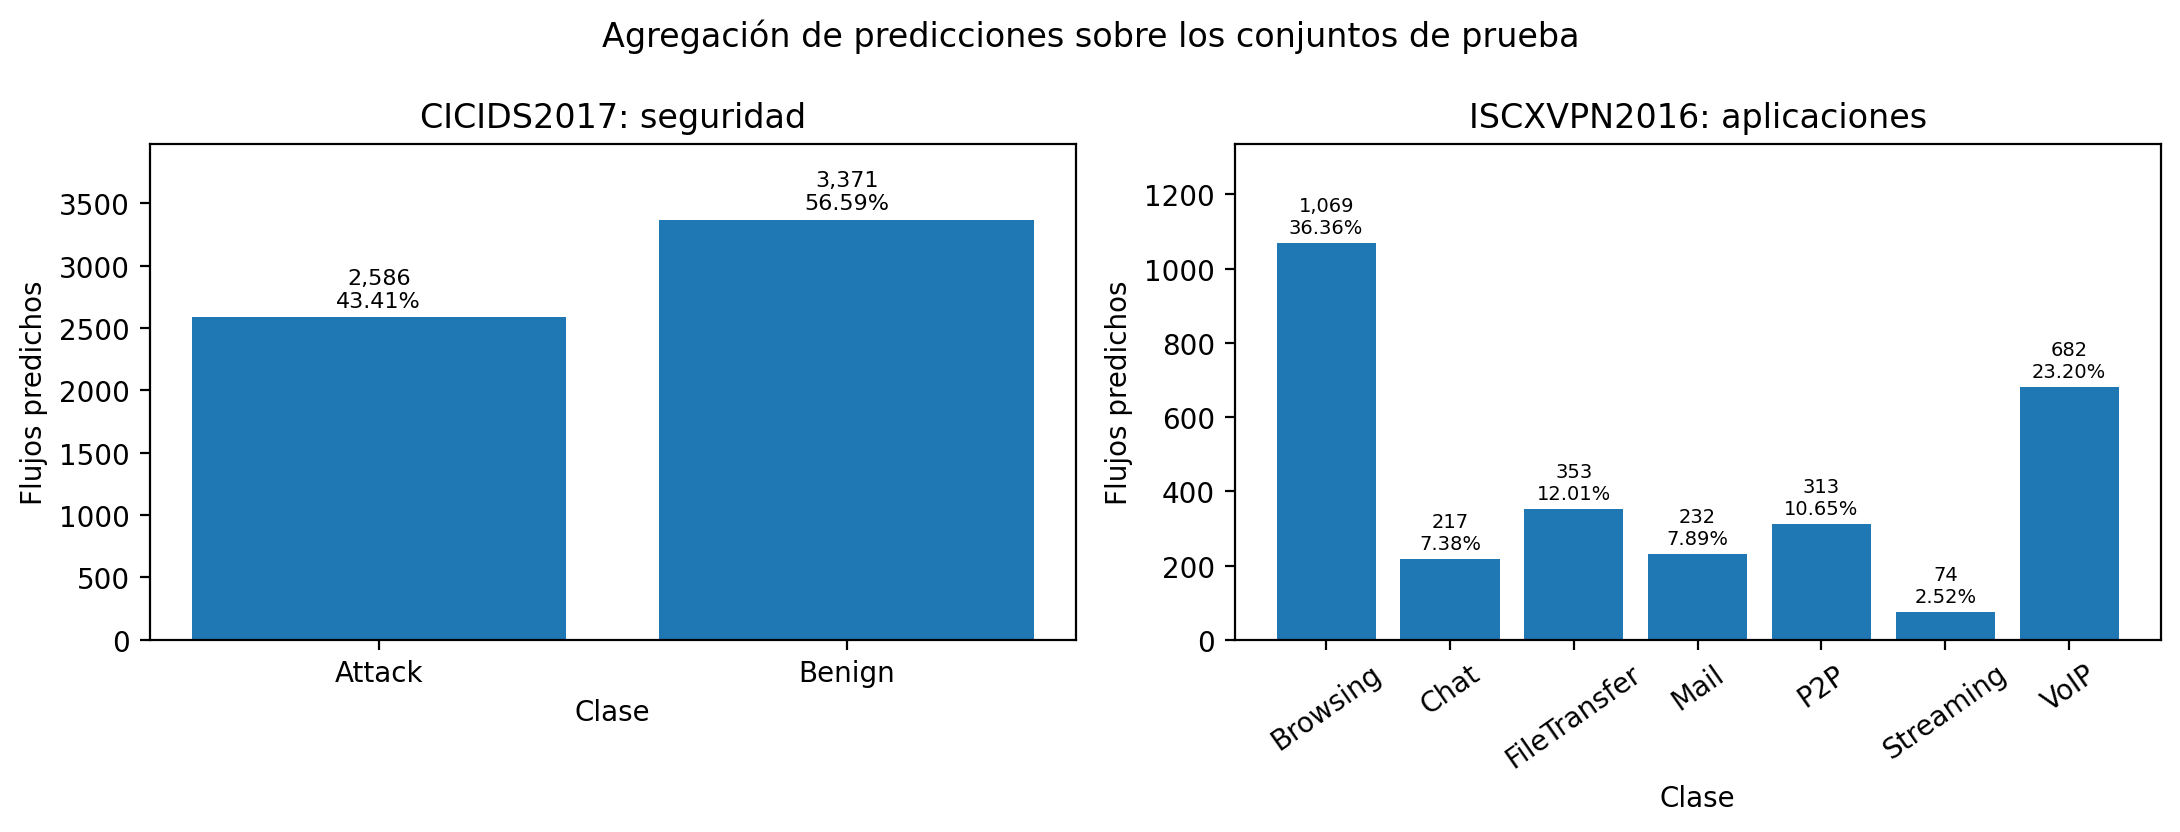
\includegraphics[width=\linewidth]{figuras/agregacion_trafico.png}}
{\fbox{\parbox{0.88\linewidth}{\centering Figura pendiente: agregación de predicciones sobre los conjuntos de prueba.}}}
\caption{Conteo de flujos por clase predicha en los conjuntos de prueba de CICIDS2017 e ISCXVPN2016. Los porcentajes corresponden a cada conjunto por separado.}
\label{fig:agregacion}
\end{figure}

\section{Alcance y limitaciones}
\label{sec:limitaciones}

\textbf{Alcance.} El proyecto abarcará la clasificación de flujos de red representados como datos estructurados y la visualización agregada de resultados. Se estudiará un número acotado de categorías de aplicaciones/servicios y, sobre un único dataset de seguridad, un conjunto delimitado de categorías relacionadas con seguridad.

\textbf{Límite de identificación.} El sistema no se presentará como un mecanismo capaz de identificar de forma determinista cualquier aplicación a partir de su IP. Las IP, puertos y datos DNS se tratarán como atributos contextuales y la salida del modelo se interpretará como una clasificación con incertidumbre.

\textbf{Límite de seguridad.} Una clasificación de seguridad no se interpretará automáticamente como prueba de malware, intrusión o intención maliciosa. Las etiquetas dependerán de la definición de los datasets y del alcance experimental.

\textbf{Límite de generalización.} Los resultados obtenidos con un dataset público no se extrapolarán directamente a cualquier red real. Las diferencias de ambiente, aplicaciones, protocolos y distribución de datos pueden reducir el desempeño fuera del dominio de entrenamiento \cite{shen2023,liang2024,pathmaperuma2022,arp2022}.

\textbf{Limitaciones de CICIDS2017.} Es un conjunto de referencia generado en un entorno controlado; su distribución de ataques y características puede no representar redes actuales y presenta problemas documentados de etiquetado, captura y construcción de flujos \cite{engelen2021,lanvin2022,rosay2022,ring2019}. La muestra usada es balanceada (20\,000 flujos por clase), de modo que sus métricas no reflejan la prevalencia natural de ataques, en la que predomina el tráfico benigno. Excluir los puertos y el protocolo no elimina otros posibles sesgos propios del dataset. La partición por intervalos de diez minutos es aleatoria entre grupos y no equivale a una evaluación entre días distintos; además, la proporción de ataques varía por día de captura (Tabla~\ref{tab:dias}), por lo que el modelo podría aprovechar rasgos asociados al momento de captura. Finalmente, los falsos negativos (98 ataques no detectados en la prueba) son una limitación relevante para una aplicación de seguridad.

\textbf{Limitaciones de ISCXVPN2016.} Se empleó una única configuración (ventana de 60 segundos, variante \texttt{AllinOne}), por lo que los resultados no se extienden a las demás ventanas. Las categorías tienen soportes muy distintos (Streaming tiene 84 registros de prueba frente a 993 de Browsing) y el recall de Chat y Streaming es menor al de las demás categorías. La tarea es identificación de aplicaciones o servicios, no detección de VPN. Al no disponer de identificador de sesión, la partición estratificada puede ser optimista, y la generalización a tráfico contemporáneo requiere validación adicional \cite{arp2022,drapergil2016}.

\textbf{Privacidad.} La captura propia se limitará a un entorno bajo control del investigador y se evitará almacenar contenido de comunicaciones cuando no sea necesario. El objetivo será trabajar con metadatos de flujo y variables estadísticas.

\textbf{Enriquecimiento activo de destinos (fuera de alcance).} Se consideró la posibilidad de resolver la categoría de flujos no reconocidos mediante consultas activas al destino observado (p. ej. cargar el sitio o el recurso asociado). Esta técnica queda deliberadamente fuera del alcance del proyecto: introduce una fuente de información activa e inconsistente con el diseño basado en metadatos pasivos, no es aplicable a los datasets públicos utilizados para entrenamiento, y plantea consideraciones adicionales de tiempo, alcance ético y viabilidad técnica que exceden lo razonable para un proyecto de un semestre. Se documenta como una posible línea de trabajo futuro, restringida a fines de interpretación y no de clasificación.

\section{Producto esperado y despliegue}

El resultado esperado será una aplicación web desplegada en la nube con una arquitectura mínima formada por una interfaz de usuario, una API de inferencia y un componente de clasificación que cargue el modelo previamente entrenado. El prototipo permitirá presentar un conjunto de flujos y obtener su clasificación, además de generar una vista agregada del tráfico analizado. La Tabla~\ref{tab:componentes} detalla los componentes previstos y su función.

\begin{center}
\small
\textsc{Cliente web} $\rightarrow$ \textsc{API} $\rightarrow$ \textsc{Preprocesamiento} $\rightarrow$ \textsc{Modelo ML} $\rightarrow$ \textsc{Clasificación} $\rightarrow$ \textsc{Agregación / visualización}
\end{center}

\bibliographystyle{IEEEtran}
\bibliography{references}

\end{document}
